\documentclass[12pt,a4paper]{article}
\usepackage[utf8]{inputenc}
\usepackage{graphicx}
\usepackage[margin=1in]{geometry}
\usepackage{lscape}
\usepackage{pgfplots}
\usepackage{setspace}
\usepackage{pgfgantt}
\usepackage{listings}
\definecolor{dkgreen}{rgb}{0,0.6,0}
\definecolor{gray}{rgb}{0.5,0.5,0.5}
\definecolor{mauve}{rgb}{0.58,0,0.82}

\lstset{frame=tb,
  language=Java,
  aboveskip=3mm,
  belowskip=3mm,
  showstringspaces=false,
  columns=flexible,
  basicstyle={\small\ttfamily},
  numbers=none,
  numberstyle=\tiny\color{gray},
  keywordstyle=\color{blue},
  commentstyle=\color{dkgreen},
  stringstyle=\color{mauve},
  breaklines=true,
  breakatwhitespace=true,
  tabsize=4
}

\graphicspath{ {images/}}
\begin{document}
\thispagestyle{empty}
\begin{figure}
\centering
\begin{minipage}{.5\textwidth}
  \centering
  
\includegraphics[width=.7\linewidth]{hwlogo}
  \label{fig:test1}
\end{minipage}%
\begin{minipage}{.5\textwidth}
  \centering
  
\includegraphics[width=\linewidth]{roboticslogo}
  \label{fig:test2}
\end{minipage}
\end{figure}
{
\centering
\vspace{10mm}
{\huge Evolving a Learning Agent using Neuroevolution in the FightingICE Game Framework}\\
\vspace{20mm}
{\large Final Year Dissertation}\\
{\large Heriot-Watt University}\\
\vspace{10mm}
{\large Robert John Dunn\\
H00163867\\
BSc Honours in Computer Science\\
}
\vspace{10mm}
{\large Supervisor:}\\
Dr Patricia A. Vargas\\
School of Mathematical \& Computer Sciences\\
Heriot-Watt University
\vspace{3mm}\\
{\large Co-Supervisor:}\\
Dr Fabrício Olivetti de França\\
Center of Mathematics, Computing and Cognition\\
Federal University of ABC, Sao Paulo, Brazil
\vspace{3mm}\\
{\large Second Reader:}\\
Dr Mohamed Abdelshafy\\
School of Mathematical \& Computer Sciences\\
Heriot-Watt University\\}
\newpage
\thispagestyle{empty}
\vspace*{30mm}
\section*{Declaration}
I,  Robert Dunn confirm that this work submitted for assessment is my own and is expressed
in my own words. Any uses made within it of the works of other authors in any
form (e.g., ideas, equations, figures, text, tables, programs) are properly acknowledged
at any point of their use. A list of the references employed is included.\\

Signed: Robert John Dunn\\

Date: 03/05/2017
\newpage
\thispagestyle{empty}
\begin{abstract}
Neuroevolution is a popular technique for machine learning in which the topology and/or weights of an artificial neural network are adjusted by an evolutionary algorithm. The technique takes inspiration from the evolution of the biological nervous system and is a popular approach for reinforcement learning problems. One way to demonstrate the effectiveness of neuroevolution is through artificial intelligence in games. This project aims to implement a learning agent in the FightingICE platform, a two-dimensional Java fighting game organised and maintained by Ritsumeikan University, Kyoto. The agent is designed to evolve through neuroevolution to improve its performance in the game, eventually becoming competitive versus a human opponent. By implementing a neuroevolution method in a simplistic environment, we hope to evaluate the effectiveness of neuroevolution as a method of machine learning and explore the potential of our agent's performance.
\end{abstract}
\newpage
\thispagestyle{empty}
\tableofcontents
\newpage
\section{Introduction}
\subsection{Motivation}
\onehalfspace
The ability to learn is a fundamental attribute of intelligent behaviour which is possessed by humans, animals, and even plants. The learning processes include the acquisition and organisation of new knowledge, the development of motor and cognitive skills, and the discovery of new facts and theories \cite{michalski}. This provides us with the ability to overcome many challenges and difficulties we encounter, as well as providing the information we need to survive in an ever-changing environment which has made us who we are today.\\

The field of Artificial Intelligence is the study of emulating intelligence within machines, also known as the study of 'intelligent agents'. The field aims to give machines the ability to learn, as well as other abilities considered intelligence such as having reasoning and being able to represent knowledge. Studies into providing an agent the ability to learn usually focus on a specific problem. The agent can then be trained to complete the specific task successfully and will have successfully emulated the learning process.\\ 

The field of machine-learning aims to imitate this learning attribute and apply it to machines in order to improve their performance at tasks without being explicitly programmed. Machine learning methods do not aim to mimic the human learning process exactly but are often inspired by it. Representing the process in a computational model involves the agent learning to cope with specific problems by using observable or measured data and statistical or mathematical approaches.\\

One application of machine learning often studied is the the creation of intelligent agents which utilise a machine learning method. The method is often applied to the autonomous agent to improve its performance at dealing with a specific task.\\

A possible environment to implement these intelligent agents in is that of a traditional or video game. Games are a particular interesting application area due to the fast decision making and acknowledgement of a complex scenario needed.\\

A recent game created for the allowance of implementing intelligent agents is the FightingICE game framework. The framework was developed in Java by the Intelligent Computer Entertainment Lab at Ritsumeikan University, Japan. The game itself involves two characters fighting versus each other in an arena- similar to popular fighting games such as Tekken and Street Fighter. The framework provides interfaces and methods to ease implementation of agents in it.\\

One machine learning approach often used is that of artificial neural networks (NN). Artificial neural networks are inspired by the biological nervous system: collections of neurons communicating with each other through axons.\\

Common learning algorithms for a NN such as back-propagation depend on knowing specific (input, target) pairs, though this information is not always available. Some problems only provide information on how well a NN has performed after a sequence of inputs, learning based on feedback of its performance.\\

One such method requiring only feedback about its performance to learn is neuroevolution. Neuroevolution is inspired by the biological brain, which has been evolved over time through natural selection. The method uses an evolutionary computation algorithm to optimise parameters of an NN.\\

From this work we hope to evaluate the effectiveness of the neuroevolution method for this particular problem. We also hope to improve our understanding of the learning process by answering whether incrementally more complex scenarios benefit the learning and whether it is possible to evolve an agent to the point of being competitive versus a human opponent, though not overly so.\\

Hypotheses:
\begin{itemize}
\item {H1: The agent's evolution will benefit from the introduction of incrementally more complex scenarios.}
\item {H2: Neuroevolution will be able to evolve the agent to a stage of being competitive versus a human opponent.}
\end{itemize}


\newpage
\subsection{Objectives}
This project aims to implement a neuroevolution algorithm acting on a learning agent in the FightingICE game platform. The inputs to the algorithm will be based on the agent's environment, such as the enemy's current position and the enemy's energy level, the outputs will be character actions e.g. move left, move right, attack. In order to increase the rate of the agent's evolution, an environment using incremental evolution will be used, exposing the agent to progressively more difficult challenges.\\

Once implemented, we will evaluate the algorithms performance versus a human opponent. Agents from different stages of evolution will be tested versus the the opponent in order to evaluate the beneficial effect the evolution has on the agent's performance. We will also compare the effectiveness of the algorithm to that of previous prototypes to evaluate any improvements made.\\

From this project, we hope to assess the effectiveness of neuroevolution as a method of machine-learning and gain the programming experience from implementing it. We also hope to find the potential to which an agent employing a neuroevolution method to learn can perform. Through comparisons of the algorithm to previous prototypes, we can also assess the progress of our algorithm over time and how improvements affect the agent's performance. The dissertation objectives are listed below in the form O1, O2...\\

\begin{itemize}
\item {O1: Implement an artificial neural network in the FightingICE game framework.}
\item {O2: Implement the neuroevolution method to evolve an agent in the game.}
\item {O3: Implement an incremental learning environment for the agent and assess the truth of hypothesis 1 (H1) by evaluating evolution data from one agent who utilises the environment and one which doesn't.}
\item {O4: Evaluate the agent's performance versus an opponent. We will implement multiple difficulties of agents and test them versus the human, using the resultant data to assess the truth of H2.} 
\end{itemize}
\newpage
\subsection{Professional, Legal, Ethical and Social Issues}
\subsubsection{Professional Issues}
A professional mindset will be employed when approaching this project. The mindset will involve appropriate communication with staff on the project and meeting deadlines reliably. Drafts will also be provided to the project supervisor with suitable time to provide feedback. When dealing with human participants for the agent testing, care will be taken to anonymise the participants data and ensure the data is protected accordingly.

\subsubsection{Legal Issues}
In order to avoid any legal issues during the project, we will ensure that any code or external work used is correctly referenced and the work holds an appropriate sharing license. This should prevent any copyright claims from outside sources. Since the project is a dissertation project for Heriot-Watt University and is purely for research purposes, there is not likely to be any legal issues arising.

\subsubsection{Ethical and Social Issues}
The majority of this project will be completed within a controlled, software-development environment, where ethical and social issues are of no concern. When human participants are involved for the agent evaluation, care will be taken to keep the environment safe and risk-free. Since only the use of a computer is involved for the evaluation, there are few potential risks.
\newpage
\section{Literature Review}
In this section of the dissertation, we will present any fundamental concepts used in the project. We will also discuss and evaluate relevant work in the field.
\subsection{Machine Learning}
Learning is a fundamental human function in which we modify our behaviour tendency according to experiences or teaching \cite{michalski}, to become better when a similar situation occurs. In the study of machine-learning, algorithms, computer applications, and systems, utilise learning to improve their performance at certain tasks. There are two main entities in the machine-learning model, the teacher and the learner. The teacher, while not always available, contains the knowledge to perform a given task while the learner has to learn the knowledge the teacher holds. \cite{swarmann}\\

There are multiple methods of learning used in the field of machine learning which define how the learner and the teacher communicate. The most common being supervised learning, unsupervised learning, and reinforcement learning. These methods describe how information is passed between the learner and teacher, and in which way the learning process is mimicked.\\

Supervised learning is when the teacher supervises the learning process, providing the learner the ability to infer the function after being provided training data. A teacher provides the learner with a set of input and desired output pairs. The learner can then use these examples to improve its performance at the task. A machine-learning method is employed to train the learner with this data, causing it to learn to approximate the function when given real input.\\

Unsupervised (also known as self organised) learning consists of only a learner and no teacher. Data is provided to the learner though unlike supervised learning, there is no labelled response associated. There is no teacher, so the learner learns based only on the observed relationships. A common application is finding patterns or grouping within data, using methods such as cluster analysis, where clusters are modelled based on measures of similarity.\\

Finally, reinforcement learning consists of a learner being given reward based on its performance. The agent uses goal-directed learning where a notion of reward is introduced and the agent attempts to maximise this reward. There is no teacher for the agent and no explicit model of the environment. Reinforcement learning can be seen as a computational approach to learning from interaction. \cite{reinforce}
\newpage
Another way to categorise machine learning methods is regarding the task performed by the method.\\

Classification tasks are commonly used and involve the agent mapping input to discrete categories, an example of pattern recognition. An agent which can successfully complete a classification task is referred to as a Classifier. In order to train itself to classify input data, data sets consisting of patterns and correct classifications are provided to the agent. The agent then adapts itself to map each input to the correct output category, effectively learning. Some real-world problems tackled by classifiers include spam detection in emails, face recognition software, biometrics, and medical diagnosis. \\

Regression tasks are similar to that of classification, though with continuous outputs instead of discrete categories. Regression is a supervised task where training data is provided to the agent of correct input-output pairs. Applications of regression agents include predicting the value of stock in the financial world, predicting weather through temporal trends, and epidermiology.\\

Clustering is the process of assigning different inputs to different groups, as classification is, though unlike classification the groups are not defined beforehand. Clustering is typically an unsupervised learning task.\\

Various methods of machine-learning exist which allow the agent (machine) to adapt itself in order to process new data. One of these methods is neuroevolution, which involves the weights and/or topology of an artificial neural network being adjusted by an evolutionary algorithm. The neuroevolution method is loosely based on the way the biological nervous system operates: with neurons communicating through axons, represented by nodes of the neural network with weighted connections. Neuroevolution has received huge popularity due to the fact that many artificial intelligence problems can be cast as optimisation problems, and since the method is ground in biological metaphor and evolutionary theory. \cite{risi}\\

\newpage
\subsection{Artificial Neural Network and Neuroevolution}
\subsubsection{Artificial Neural Network}

Artificial neural networks model the way the brain solves problems with collections of neurons communicating through axons, represented with nodes of the network with weighted connections. \\

The most basic version of an ANN (artificial neural network) is a perceptron. A perceptron is a simple machine which takes a variable number of input nodes which connect to a single output node. \cite{percept} The concept of the perceptron was extended by means of the the multi-layer feed forward network, which incorporates extra 'hidden' layers of nodes between the input and output. The more hidden layers there are, and the more nodes in these layers, the more complex behaviour a network can experience. \cite{ffann}\\

Neural networks can be employed in a variety of ways, for both supervised and unsupervised/reinforcement learning problems. Networks can have an associative (content-addressable) memory and can also implement parallel processing across individual nodes. \cite{nnm} Common applications for neural networks include character recognition, image compression and stock market prediction. \cite{nnapps}
\begin{figure}[h]
\centering{
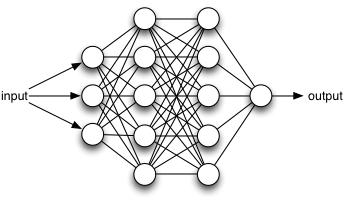
\includegraphics[width=0.8\textwidth]{ann}
\caption{Multi-layer feed forward artificial neural network.}
}
\end{figure}
\newpage
In order to calculate the output of a certain node in a network given the input or set or inputs, we use an activation function. \cite{activate} This output of the node is usually saturated to a value between minus and positive one by the function and then scaled appropriately when output. \cite{swarmann} \\

The simplest activation function is the step function \cite{nnm}, where if the weighted sum of the inputs to the node falls below a certain threshold the output is zero, else the output is one. This can be thought as the node either sending signals or not sending signals. The step function is used in perceptrons and often shows up in other models. \cite{percept} Since there are only two possible outputs of nodes using the step function, it is common to use different, more general functions.\\

One of these more general, non-linear activation function is the hyperbolic tangent function tanh, shown in figure 2. This allows nodes to have an activation output of a real number between negative one and one. The usage of these more general functions allows us to exhibit more complex behaviour within the network.
\begin{figure}[h]
\centering{
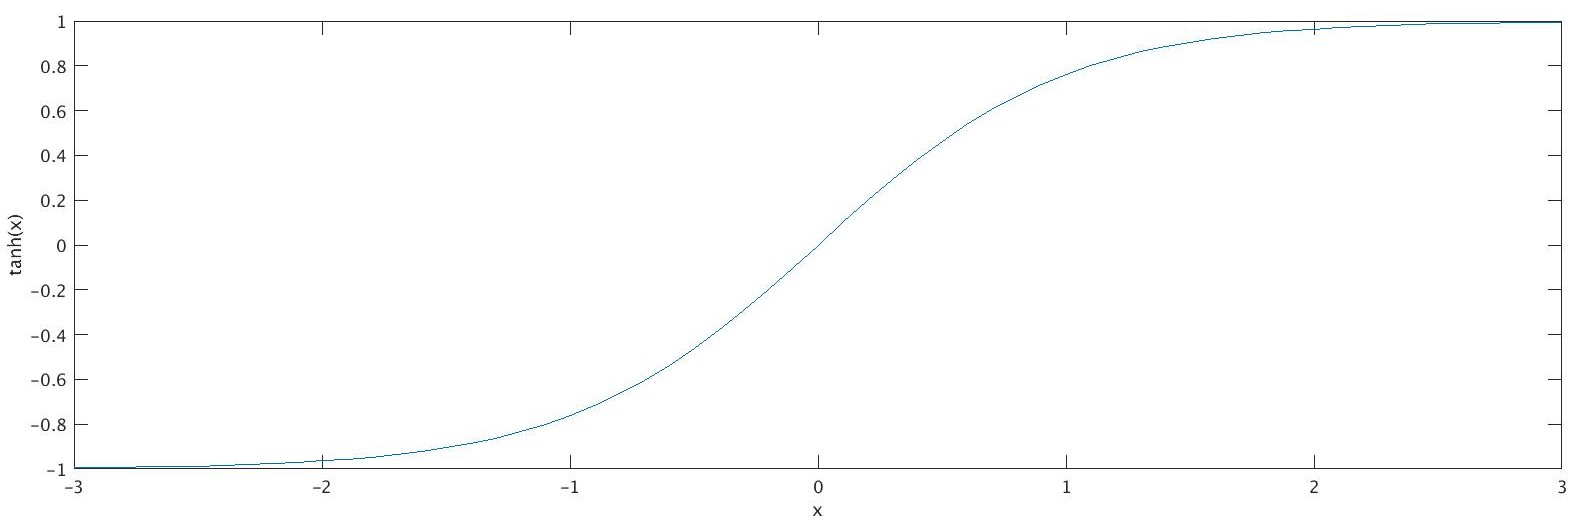
\includegraphics[width=0.6\textwidth]{tanh}
\caption{Hyperbolic tangent function plot.}
}
\end{figure}
\newpage
\subsubsection{Evolutionary Algorithms}
Evolutionary algorithms are methods of optimisation, where potential solutions to the problem are seen as individuals of some population. Each individual in the population is assigned a fitness value which is calculated according to the performance of the provided solution, and the algorithm works to find the best (fittest) of these solutions. Using techniques inspired by biological evolution such as reproduction, mutation, recombination, and selection, new populations of solutions can be generated and assessed. Using evolutionary algorithms allows fine tuning of the search space through constants such as rate of reproduction and mutation rate \cite{gas}. Pseudocode for the application of an evolutionary algorithm is shown in Listing 1.\\
\begin{lstlisting}[caption=Evolutionary algorithm pseudocode]
population = initialisePopulation();
evaluatePopulation(population);
While (stopCondition != true) 
	childPopulation = initialiseChildPop();
	parents = selectParents(population);
	For (parent In parents)
		child1, child2 = crossover(parent0, parent1);
		child1 = mutate(child1);
		child2 = mutate(child2);
		childPopulation.add(child1);
		childPopulation.add(child2);
	End For
	evaluatePopulation(childPopulation);
	population = replace(childPopulation);
End While
\end{lstlisting}

\vspace{4mm}

The algorithm begins with an initial population of random individuals being generated. The performance of each individual in the population is then evaluated, with each individual being assigned a fitness depending on how effectively they completed the task. Parents used to create the next generation are selected and reproduce (crossover) to create two children. A mutation operator is then applied to these children and the algorithm evaluates this population to then repeat the cycle. The algorithm runs until either a defined number of generations have passed or until the fitness has converged to a predetermined point.\\
\newpage
\subsubsection*{Genotype Representation}
Genotypes (also known as chromosomes) in an evolutionary algorithm hold the parameters which define a solution to the problem. Genotypes are often represented as a binary string of 1s and 0s, though other data structures can be used. A genotype defines the limitations of the search space in the algorithm. Mutation and crossover operators used in the algorithm will need to take account of the representation used. An example of a genotype representation is shown in figure 3, where real values are usually used to represent weights of an artificial neural network.\\

\begin{figure}[h]
\centering{
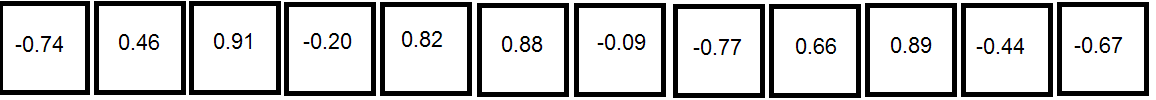
\includegraphics[width=\textwidth]{tsp}
\caption{Example genotype representation for the weights of an artificial neural network. Each gene refers to the value of an individual weight in the network.}
}
\end{figure}

\vspace{3mm}

\subsubsection*{Selection Operator \& Selective Pressure}
The selection operator in an evolutionary algorithm is used to choose appropriate genotypes for breeding from a population. The selection operator usually tries to pick higher fitness individuals for breeding over others, this is called selective pressure. The idea being that high fitness individuals will produce offspring of a high fitness.\\

Some popular selection operators include fitness proportionate selection in which parents are selected based on their fitness as a proportion of the total population's fitness. Another being tournament selection in which individuals compete versus other candidates in a tournament fight, with the highest fitness individual winning.\\

\subsubsection*{Crossover Operator}
The crossover operator is used to breed new individuals to create a new population of solutions. The operator involves applying crossover to two parents (reproduction) in order to create two child genotypes. Crossover creates variety between solutions and promotes the generation of fitter future generations.\\
\newpage
One method of crossover is single-point crossover in which a single point of each parent's genotype is chosen. The first child generated consists of the genotype of the first parent up until the determined crossover point and then the rest of the second parent's genotype. The second child being likewise though with the parent's roles swapped.\\

Another crossover operator is two-point crossover. In this approach, two points are chosen on each parent genotype. The first child is then generated by swapping the section between the points of the first parent into the second parent, and likewise for the second child. An illustration of an implementation of two-point crossover can be seen in figure 4.\\

\begin{figure}[h]
\centering{
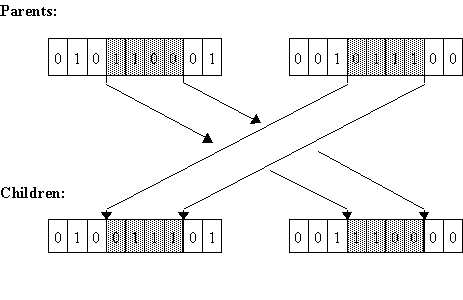
\includegraphics[width=0.7\textwidth]{crossover}
\caption{Illustration of two-point crossover.}
}
\end{figure}
\subsubsection*{Mutation Operator}
The final operator is the mutation genetic operator. When mutation occurs to genotypes, one or more genes within the chromosome are 'mutated' to a new value. The use of mutation keeps genetic diversity in the population, preventing us from hitting local plateaus and periods of slow evolution. A common method of mutation is bit string mutation, in which genes in a binary string are flipped at random (1 to 0 and 0 to 1). Another method, common for use with artificial neural networks, is to update the mutated gene to a new random value within the weight range (which is usually -1,1).
\newpage
\subsubsection{Neuroevolution}
Neuroevolution is a biologically-inspired method of machine learning in which an artificial neural network is evolved using an evolutionary algorithm. The biological inspiration for the method comes from the nervous system in which neurons communicate through axons, translated to machine-learning by the nodes of a neural network communicating through weighted connections. The method has proved popular, especially in the fields of artificial life, evolutionary robotics and computer games. One reason for its popularity is the fact that neuroevolution is a form of reinforcement learning, which can be applied more generally than its counterpart, supervised learning. The popularity also stems from the fact that the method is ground in biological metaphor and evolutionary theory. The method consistently performs well in many areas of application and can handle large action/state spaces. \cite{risi}\\

The applications of neuroevolution are numerous and diverse. One application is the implementation of artificially intelligent agents in computer games (see section 2.2.5). Other applications include dynamic resource allocation, optimising manufacturing processes and even creating musical melodies. \cite{neapps}
\begin{figure}[h]
\begin{center}
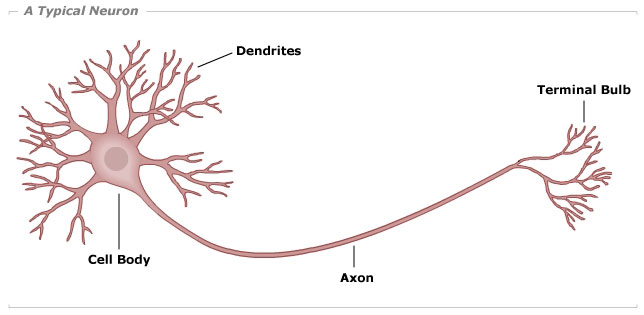
\includegraphics[width=0.6\textwidth]{neuron}
\caption{Annotated diagram of a biological neuron.}
\end{center}
\end{figure}
\vspace{-7mm}
\subsubsection{Incremental Evolution}
When an agent is provided with a complex behaviour, it may have trouble evolving to perform at its potential. Using incremental evolution, the behaviour can be learnt incrementally with tasks gradually increasing in difficulty. This form of evolution proved effective in at least one implementation \cite{incre}. The agent's task was a prey capture task: the agent moves through the environment and must catch its prey before the set number of time-steps. With increasingly difficult tasks, the agent was able to rapidly improve its performance, and skip many potential generations of evolution. We hope to experiment with the usage of incremental evolution in our project to assess whether it has a positive impact on the evolution of the agent.
\newpage
\subsection{FightingICE Game Platform}
FightingICE is a Java based game platform organised and maintained by Intelligent Computer Entertainment Lab., Ritsumeikan University. The game is based in an arena where two fighters are competing versus each other, attempting to deplete the other's hit-points while preserving their own.\\ 

The FightingICE platform was designed to allow easy development and evaluation of artificially agents in the game for research or hobby purposes. Once implemented, an agent receives information about the state of the game from the platform periodically, such as the opponent player's location and current energy levels. A delay is added to this game information in order to simulate the delay a human player would experience from reaction time. \cite{fightingice}\\

\subsubsection{Learning Environment}
There are four characters available in the game: Zen, Garnet, Lud, and Kfm. Each of the characters is capable of moving, performing attacks, and combining these attacks into unique combos. The game starts with each player at 0 hit-points and 0 energy. Once a player successfully connects an attack against its opponent, the player's energy is increased and the opponent's hit-points decrease. In order to compete against an opponent, the character must dodge opposing attacks and make effective use of energy to land attacks and reduce the opponent's hit-points.\\
\begin{figure}[h]
\centering{
\includegraphics[width=0.8\textwidth]{fightingICE}
\caption{Screenshot of the FightingICE platform in action.}
}
\end{figure}
\newpage
\subsection{Related Work}
When implementing neuroevolution, a computer game is a common choice of environment. Neuroevolution methods have been used as artificial intelligence in games in the following external projects:
\begin{itemize}
\item Improving AI for simulated cars. \cite{pace}
\item Neuroevolution approach to general video game playing. \cite{genvid}
\item Calculating optimal jungling routes in the game DOTA2. \cite{dota}
\item Using neuroevolution to play atari games. \cite{atari}
\end{itemize} 
The work has found neuroevolution to be an effective machine-learning algorithm in a computer game environment and the method proved to operate consistently across a diverse range of games.\\

There are also numerous agents programmed in the FightingICE platform to compete in competitions. \cite{fightingice} We will test and assess the performance of a select few agents at a later stage of this project. Hopefully from this assessment of the agents we can evaluate the strategies of the programmer to improve the agent's performance as well as the effectiveness of different methods of AI.

\newpage
\section{Organisation}
In this section we present the decision process on how to approach the task including analysis of the task itself, analysis of the requirements, and analysis of the risks. A gantt chart of the project timeline is also included.
\subsection{Project Task Analysis}
The objective of this project is to evolve an agent in the FightingICE game platform with a neuroevolution method. The agent will be evolved to the point of being competitive versus a human opponent. \\

In order to implement the neuroevolution method, we will first need an artificial neural network to control the actions of the agent. The neural network will need to take as input various factors from its environments such as the location of the opposing player, the energy of the opposing player and whether the opponent is performing an attack. The outputs of the neural network will be actions for the character, for example move left, jump, attack. Once a neural network controlling the agent has been implemented, the network must be evolved to imitate the learning process. This will involve deciding on a suitable evolutionary algorithm and the encoding of the network's genotype.\\

To improve the rate of evolution for the agent, we will create an incremental evolution environment where the agent is exposed to tasks of gradually increasingly difficulty. To implement this environment, we will limit the capabilities of the training opponent and gradually return them.\\

To test whether the agent's performance has improved to the point of being competitive versus a human opponent, we will find volunteers of varying skills to face our agent in the game. The results of the player versus our agent at various stages of its evolution can then be evaluated to assess the effectiveness of the neuroevolution algorithm which we implemented.
\newpage
\subsection{Requirement Analysis}
\subsubsection{Table of Requirements}
\begin{tabular}{|p{0.1\linewidth}|p{0.5\linewidth}|p{0.1\linewidth}|p{0.2\linewidth}|}
\hline
No. & Requirement & Priority & Predecessors\\ \hline
1 & Implement a neural network to control agent's behaviour & High &\\ \hline
1.1 & Initialise a network with random weights, test if the sensors can be read and the actions can be output & High &\\ \hline
1.2 & Implement a simple rule-based agent for the agent to compete versus & High & 1.1\\ \hline
1.3 & Test and execute at least one agent from the FightingICE AI competition & Medium &\\ \hline
2 & Implement an appropriate evolutionary algorithm to evolve the neural network & High & 1\\ \hline
2.1 & Test whether a simple evolutionary algorithm evolving the weights of the network improves the agent's performance & High & 1\\ \hline
3 & Create an incremental evolution environment for the agent & Medium & 1, 2\\ \hline
3.1 & Limit the capabilities of the opponent and incrementally return them to test whether speed of evolution is improved & Medium & 1, 2\\ \hline
3.2 & Evolve against a simple agent, replace opponent with best agent after convergence and continue & Medium & 1, 2\\ \hline 
4 & Evaluate the agent's performance versus a human opponent at various stages of its evolution & High & 1, 2\\ \hline
\end{tabular}
\newpage
\subsubsection{Requirements Textual Descriptions}
\subsubsection*{1 - Implement a neural network to control agent's behaviour}
To implement an agent in the FightingICE platform controlled by a simple neural network.
\subsubsection*{1.1 - Initialise network with random weights, test if sensors can be read and actions can be output}
In order to test whether sensors can be read and actions can be output, initialise a simple neural network with random weights to control the agent. Ensure game information is being received and number of outputs nodes match character actions.
\subsubsection*{1.2 - Implement a simple rule-based agent for the agent to compete versus}
Create agent in FightingICE which follows simple rule-based logic. Use as an opponent for the neuroevolution agent while it is evolving.
\subsubsection*{1.3 - Test and execute at least one agent from the FightingICE AI competition}
Find agents from the FightingICE AI Competition and test them to see strategies of other programmer's work. Attempt to read and understand the code.
\subsubsection*{2 - Implement an appropriate evolutionary algorithm to evolve the neural network}
Find and implement an appropriate evolutionary algorithm to evolve the ANN of the agent. Decide on implementation based on performance evaluation.
\subsubsection*{2.1 - Test whether a simple evolutionary algorithm evolving the weights of the network improves the agent's performance}
Implement a simple EA such as hill-climbing or an algorithm using only mutation to evolve the agent's neural network. Test whether the evolution improves the agent's performance and if so, to what extent.
\newpage
\subsubsection*{3 - Create an incremental evolution environment for the agent}
Create an incremental evolution environment to speed the process of evolution for the agent.
\subsubsection*{3.1 - Limit the capabilities of the opponent and incrementally return them to test whether speed of evolution is improved}
Initially, completely limit the capabilities of the agent's opponent and gradually return these capabilities over time. Evaluate whether gradually exposing the agent to these capabilities improved the speed of evolution of the agent.
\subsubsection*{3.2 - Evolve against a simple agent, replace opponent with best agent after convergence and continue}
Begin evolution with simple rule-based opponent. Once convergence in evolution occurs, replace the agent's opponent with the current best agent. Repeat this process incrementally and compare performance of each opponent with that of its successors.
\subsubsection*{4 - Evaluate the agent's performance versus a human opponent at various stages of its evolution}
Test the performance of different agents at different stages of their evolution against human players. Attempt to find volunteers that rank at different skill levels from novice to expert. From this we can assess whether the agent was evolved to become competitive versus a human opponent.

\newpage
\subsection{Performance Assessment}
\subsubsection{Table of Project Prototypes}
\begin{tabular}{|p{0.4\linewidth}|p{0.2\linewidth}|p{0.4\linewidth}|}
\hline
Objective & Date & Assessment\\ \hline
Prototype 1: Agent using neural network to sense environment and output simple actions in FightingICE & 15/12/2016 & Agent can proficiently perceive its environment and output simple actions\\ \hline
Prototype 2: Agent controlled by neural network being evolved by simple evolutionary algorithm, altering only the weights of the network & 20/01/2017 & Evaluate agents performance versus simple AI opponent at different stages of its evolution\\ \hline
Prototype 3: Agent with appropriate learning method implemented in incremental evolution environment & 10/03/2017 & Agent's environment is adapted to utilise incremental evolution. Agent's performance assessed and compared versus learning without incremental environment.\\ \hline
\end{tabular}
\newpage
\subsubsection{Prototypes Textual Descriptions}
\subsubsection*{Prototype 1}
The initial prototype will involve an agent using an artificial neural network to test if the agent's environments can be sensed and the agent can output actions on the platform. Once we have evaluated the agent's functionality we will move towards evolving the neural network.

\subsubsection*{Prototype 2}
The second prototype will implement a simple evolutionary algorithm in order to alter the weights of the neural network. With an appropriate fitness function for the agent, this method of evolution should result in improvement of the agent's performance. The agent's performance versus both a simple rule-based opponent and a human opponent will be evaluated.

\subsubsection*{Prototype 3}
The final prototype for the project will utilise incremental evolution techniques to improve its rate of evolution. This prototype is due to be finished by the 10th March 2017 and will mark the end of our agent development. Once the final prototype has been completed, evaluation of the agent's performance will commence.
\newpage
\subsection{Risk Assessment}
\subsubsection{Table of Risks}
\begin{tabular}{|p{0.1\linewidth}|p{0.4\linewidth}|p{0.2\linewidth}|p{0.3\linewidth}|}
\hline
No. & Risk Name & Probability & Response\\ \hline
1 & Laptop failure & Low & Online storage (github), backups\\ \hline
2 & Difficulties with Java programming & Low & Spend more time familiarising with language and practising\\ \hline
3 & Difficulties with FightingICE platform & Medium & Consult tutorials and relevant documentation from website\\ \hline
\end{tabular}
\subsubsection{Risks Textual Description}
\subsubsection*{1 - Laptop failure}
In the case of the laptop being used to develop the project failing, essential code or documentation could be lost. To reduce the impact of this risk, we will ensure to regularly upload the code to a online repository such as GitHUB. We will also back-up any work on external hard-drives or on the university computers.
\subsubsection*{2 - Difficulties with Java programming}
To avoid any problems with lack of Java programming expertise, we will spend time familiarising ourselves with the language before development.
\subsubsection*{3 - Difficulties with FightingICE platform}
Since there is plenty of information and lots of tutorials on agent development with the platform, we should be able to easily familiarise ourselves with it.
\subsection{Project Plan}
Figure 5 shows a gantt chart representing a timeline for the completion of the project including all prototypes, the dissertation and the project poster. With this project plan we hope to leave appropriate time to evaluate any results as well as carefully thought out prototype deadline which will result in any code problems occurring early. The plan has been shown to and approved by both the project supervisor and co-supervisor.
\newpage
\begin{landscape}
{\centering
\subsubsection{Gantt Chart}
}
\vspace{10mm}
\begin{ganttchart}[vgrid, hgrid]{1}{24}
	\gantttitle{2016}{9}
	\gantttitle{2017}{15} \\
	\gantttitle{Oct}{3}
	\gantttitle{Nov}{3}
	\gantttitle{Dec}{3}
	\gantttitle{Jan}{3}
	\gantttitle{Feb}{3}
	\gantttitle{Mar}{3}
	\gantttitle{Apr}{3}
	\gantttitle{May}{3}
	\\
	\ganttbar{Deliverable One (03/10/2016 - 24/11/2016)}{1}{5}\\
	\ganttbar{Complete Interview (24/11/2016 - 16/12/2016)}{6}{11}\\
	\ganttgroup{Prototypes}{6}{17}\\
	\ganttbar{Prototype One (24/11/2016 - 15/12/2016)}{6}{8}\\
	\ganttlinkedbar{Prototype Two (16/12/2016 - 20/01/2017)}{9}{11}\\
	\ganttlinkedbar{Prototype Three (23/01/2017 - 14/03/2017)}{12}{17}\\
	\ganttbar{Results Evaluation (15/03/2017 - 10/04/2017)}{18}{19}\\
	\ganttbar{Complete Dissertation (10/04/2017 - 24/04/2017)}{20}{20}\\
	\ganttbar{Project Poster (24/04/2017 - 19/05/2017)}{21}{23}\\
\end{ganttchart}	
\end{landscape}
\newpage
\section{Methodology and Results}
\subsection{Prototype One: Artificial Neural Network in Game Framework}
The first prototype of the dissertation was to implement an artificial neural network which takes inputs from the game framework and whose outputs correspond to agent actions in the game. With this prototype we aim to familiarise ourselves with the workings of the framework and artificial neural networks. 
\newpage
\subsubsection{Design}
In order to better understand the theory and solidify the mathematics behind neural networks, this prototype will be implemented without the use of any external Java libraries. The neural network will be a feed-forward network, meaning information will move in only one direction (forward) from the input nodes. The network will consist of three layers: an input layer, a hidden layer, and an output layer. The number of nodes in the hidden layer will later be optimised to an appropriate value through experimentation.\\

Each node in the input layer of the network will correspond to a piece of game information available from the CommandCenter class provided with the FightingICE framework. The CommandCenter provides delayed data to the AI such as positioning of both players, player energy, player hit-points and more. For this prototype, I decided to use only three inputs: the x distance between the two characters, y distance, and the agent's energy. In order to evolve a competent agent at later stages, more inputs will be included such as information about the player's current action. However since this prototype is solely to test the neural network and begin working with the game framework, I decided to keep it simple for the time being. Annotations of these inputs for the network can be seen in figure 7.\\

\begin{figure}[h]
\centering{
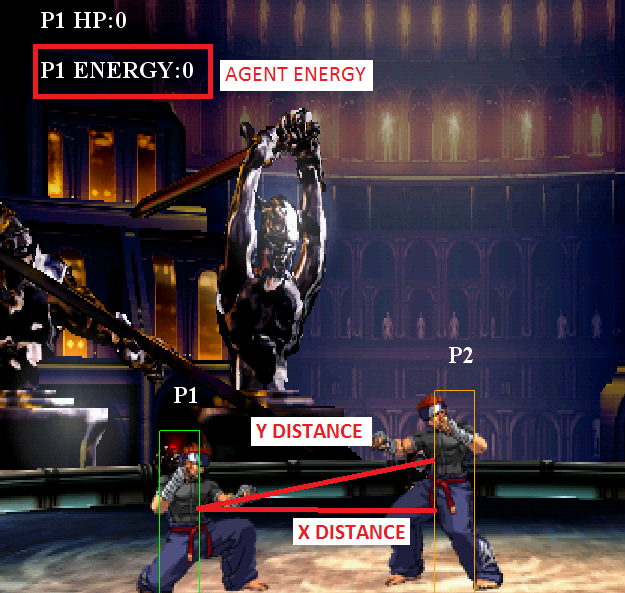
\includegraphics[height=8.5cm, width=13cm]{ANNInputs}
\caption{Labelled inputs which are taken by the artificial neural network.}
}
\end{figure}
\newpage
There will be seven output nodes for the neural network, for each of the possible actions of the agent: up, down, left, right, attack A, attack B, and attack C. The output of the network will determine whether each action is undertaken. For example, if the output nodes corresponding to right and attack A are activated, the agent will move right and attack with attack A. If the implementation is successful, the agent should exhibit different outputs (actions) based on the current state (position of both characters etc) of the game.
\newpage
\subsubsection{Implementation}

\subsubsection*{Controller}

\vspace{3mm}

The first class implemented was Prototype1 which is used to control the agent. The class implements the AIInterface interface, provided by the game framework. The interface provides methods for initialising the agent, processing game information, and sending agent outputs (actions) to the game.\\

The initialize() method initialises the various classes used by the agent. The Key object is used to output agent action and contains seven boolean variables (A, B, C, U, D, L, R) representing all possible actions. During each frame of the game, the Key object is read and the agent performs the appropriate action(s). The initialize method also initialises the FrameData object which contains information about the current game state such as frames left in the round and visual information, and the CommandCenter object which provides delayed game information to the agent with character positions and other useful data. The ANN class used for feeding for the neural network is also initialised in this method. The initialize method can be viewed in listing 2.

\vspace{5mm}

\begin{lstlisting}[caption=initialize method in Prototype1.java.]
@Override
public int initialize(GameData gameData, boolean playerNumber) {
	// TODO Auto-generated method stub
	gd = gameData;
	p = playerNumber;
	inputKey = new Key();
	fd = new FrameData();
	cc = new CommandCenter();
	ann = new ANN();
	return 0;
}
\end{lstlisting}

\newpage
Other methods used by the AIInterface include the getInformation() method which is used to set data for the FrameData object using the setFrameData() method provided from the CommandCenter object. Also included from the interface is the input() method which returns a Key object representing the agent's output, the close() method which is called when the game is closed and can be used to finalise any processing, and getCharacter() which returns the character of the agent: in this case 'CHARACTER\_ZEN'.\\

The final method used in this class is the processing() method. This method is called at every frame and is used for processing game information and determine the agent's actions. The method first ensures that frame data has been provided using the methods getEmptyFlag() and getRemainingTime() from the FrameData object. The X-distance, Y-distance and agent energy are then used to feed through the neural network with the feed() method. Before feeding, the inputs are normalised using the tanh() (hyperbolic tangent) method from the Java Math library. Feeding through the network returns an array of seven doubles, representing the output of the neural network. Following feeding through the network, variables in the Key object are set to either true or false depending on the output. Since neuron activations in the network are between minus one and one, if the output is greater than zero then the variable (action) is set to true. Once set, at the next frame when the input() method is called the agent outputs the appropriate actions.\\

\subsubsection*{Artificial Neural Network}

The next class implemented was ANN which provides methods to create an artificial neural network and feed through the network. Weights of the network are stored in two matrices of doubles: weights0 and weights1, each representing a synapse of the network (input layer to hidden layer, and hidden to output layer).\\

The class constructor initialises these matrices with an appropriate number of weights. For this prototype three input nodes were used, ten hidden layer, and seven output layer nodes. A Java Random object from the Java.util library is then used to set these weights to random values between minus one and one. The Random object provides a method nextDouble() which returns a random double value in between zero and one. In order to generate a value between minus one and one, which is needed for the neural network, this value is multiplied by two and then one is subtracted from the result.
\newpage
The sole method provided by this class, apart from the constructor, is feed() which takes three double inputs as arguments and returns an array of doubles which are the output of the network. The method initially declares and initialises two arrays of doubles to store the activations of neurons in the hidden and output layer. Next, inputs are fed through to the hidden layer by calculating the weighted sum for each node in the hidden layer using the inputs and the first synapse matrix (weights0). After, output activations are calculated: also using weighted sums however this time using the second synapse matrix, weights1. A message is printed to the standard output for each output activation for testing purposes and finally the array of doubles for the output activations is returned. A code excerpt displaying the code's functionality is seen in listing 3.

\vspace{6mm}

\begin{lstlisting}[caption=Feed method in class ANN]
/* Feed through the network with x-distance, y-distance and energy */
public double[] feed(double x, double y, double e) {
	double[] hid = new double[10];			// Hidden layer nodes
	double[] out = new double[7];			// Output layer nodes
	for(int i=0;i<10;i++) {				// Feed through to hidden layer
		hid[i] = (double) (weights0[0][i] * x			// X
			+ weights0[1][i] * y						// Y
			+ weights0[2][i] * e);						// Energy
	}
	for(int j=0;j<7;j++) {		// Feed through to output
		out[j] = 0;
		for(int k=0;k<10;k++) {
			out[j] += (weights1[k][j] * hid[k]);
		}
		System.out.println(j+"th output: "+out[j]);
	}
	return out;
}
\end{lstlisting}

\newpage
\subsubsection{Evaluation}
Since this prototype was to familiarise with the game framework and artificial neural network theory, there was no need to evaluate the agent's performance versus another artificial intelligence or human player. The agent was able to successfully read inputs from provided game data and feed through the neural network to send outputs to the game framework. This resulted in the agent's action changing based on the current game state (location of both characters and agent energy).\\

One shortcoming of the prototype was the agent only rarely attacking. This was due to the fact that if the agent attempted to output more than one attack at once (e.g. attack A and B are both activated) then they cancel each other out. In future prototypes this problem can be avoided by using if and else statements to ensure that only one attack is output at a time, regardless of whether more than one is activated in the neural network. Similarly, the agent jumped excessively due to the fact that jumping is prioritised over other movement commands. To avoid this in future prototypes, the activation needed for jump to be output can be increased to make it less likely to occur. Both problems could also potentially be avoided during the evolution of the agent, with the agent evolving to a point where it is able to avoid these conditions.\\

Other improvements which can be applied to future prototypes is with the inputs used for the neural network. Using the X and Y distance between the two characters does not allow the agent to determine whether the opponent is on its left or right side. Instead, using the x and y co-ordinates of both characters will allow the agent to adapt its behaviour based on which side of the agent the opponent is positioned. Inputs for the network should also be properly normalised and scaled. Using the hyperbolic tangent function results in values between minus one and one, as needed, though since the maximum  and minimum values of the inputs are known (e.g. minimum X co-ordinate is -120 and maximum is 680) we can properly scale and normalise them to the required range. This should provide more effective and accurate activations for the neural network, resulting in improved interactions with the agent and its environment.\\
 
A final way to improve the agent in future prototypes is to run experiments to determine the number of hidden nodes needed in the network. Since the number of input and output nodes in the network depends on the game framework, they will remain static, though different numbers of hidden layer nodes will have an impact on the effectiveness of the neural network, and therefore the agent's performance. During evolution, experiments can be run to evaluate the agent's improvement over time and determine an appropriate number of hidden layer nodes to use and optimise network parameters.
\newpage
\subsection{Prototype Two: Weights of Neural Network Evolved by Genetic Algorithm}
For the second agent prototype, an evolutionary algorithm was used to evolve the weights of the artificial neural network. This will be the first prototype to make use of the neuroevolution method. Also, the code for the neural network was rewritten in order to use the dl4j Java library.\\

The aim of this prototype is to provide the agent with the ability to train itself. With training, the agent will be able to improve its fitness (and therefore performance) in the game over time. Another aim of this prototype is to make use of the dl4j library in preparation for prototype three. The library provides any functionality that is needed for the neural network in this project and is known to be a robust and reliable library.

\newpage
\subsubsection{Design}
\subsubsection*{Artificial Neural Network}

\vspace{3mm}

The artificial neural network will be implemented using the Java library deeplearning4j (dl4j), a deep learning library for the JVM. The library provides appropriate classes to implement neural networks, as well as OpenBLAS, which provides CPU optimisations to ease use of the network and run calculations in parallel. From the dl4j library we will use the MultiLayerConfiguration and MultiLayerNetwork classes to implement our adaptation of an artificial neural network.\\

This prototype also aims to improve the processing of inputs to the neural network. In the first prototype, X and Y distance between were provided as inputs, though since the distance will always be positive it was not possible to determine whether the opponent was on the left or right side of the agent. Using the X and Y coordinates of both characters will allow the agent to determine both the distance between the two, and also the direction of the distance. Another problem in prototype one was the fact that if the agent attempted to output more than one attack at once, no attack was output. If the agent's evolution does not fix this we will implement IF-ELSE loops to only allow the agent to output a single attack per frame. This prototype will also properly scale and normalise inputs to the desired -1,1 range without the use of the hyperbolic tangent function. Since we have access to the minimum and maximum values of each variable we can properly scale them so therefore the the far left X-coordinate of the arena corresponds to an input of -1 and the far right to an input of 1.\\

\subsubsection*{Genetic Algorithm}

\vspace{3mm}

Since this prototype will be implementing the neuroevolution method, we will also need to implement a genetic algorithm which will modify (evolve) the neural network. The genetic algorithm will need to implement methods for generating the initial population as well as appropriate methods for crossover and mutation to evolve the population. A storage method for evolution data will also need to be decided.\\

Selection for crossover in the genetic algorithm will be completed using tournament selection. With tournament selection, individuals are chosen at population at random and a tournament is run of which the individual with the best fitness wins. The tournament size is predetermined and will be optimised for later prototypes. Mutation will be applied by replacing the mutated weight with a random value from the vector [-1, 1]. \\

In order to evaluate the agent's evolution and load previously evolved agents we will need a method of storing all relevant data. From inspecting other evolution projects implemented in the FightingICE framework (cite), we decided to use comma-separated values (CSV) files. The agent will create a different file for each generation of the evolution and will first write the weights of each genotype to the file. This will allow us to access previous agents and is used by the AI to update network weights. After each genotyype is run it will also write its fitness to the file to allow evolution of the population with crossover and mutation.

\subsubsection*{Parameter Tuning}

In order to optimised parameters of the neural network and genetic algorithm we will run experiments. These experiments will involve running the neuroevolution with different parameters and evaluating the speed of the agent's evolution and other relevant data. For example, the agent will be run with different population sizes to determine an appropriate value for evolution in which the population is large enough to allow for diversity within genotypes but not too large to the point of extending runtime without improving results.\\

We will also use similar experiments to determine a suitable value for the number of nodes in the hidden layer. The number of neurons will impact the complexity of the network and we aim to find an optimised value for the application of our agent. We can also determine from experiments whether three layers is sufficient for the network or more need to be added. 
\newpage
\subsubsection{Implementation}
\subsubsection*{Controller}
The first class we implemented was Prototype2, which acted as a controller for the agent. To interact with the FightingICE framework this class needed to implement the AIInterface interface and any methods included in the interface.\\

The first method included within the interface is initialize, which is used to initialise anything needed for the agent before the game begins. All Java objects used by the agent to process game information such as CommandCenter and FrameData are initialised, as well as the artificial neural network.\\

The method then checks whether the AI will be running as a demo or to evolve itself. It does this by checking for a file 'demo.txt' in the default P2EVO02 evolution directory, which is surrounded in a try/catch clause to prevent any file I/O errors. If the demo file exists, a BufferedReader object is used to parse the file and store the network weights in an array of doubles. This array is then passed to the NN's updateWeights method to set the network's weights to that of the desired demo. A code snippet for this loading of a demo is shown in listing 4.
\singlespacing
\begin{lstlisting}[caption=Loading of demo files in Prototype2 class]
File demof = new File(".\\P2EVO02\\demo.txt");
if (demof.exists() && !demof.isDirectory()) {
	try {
		System.out.println("Initialising demo");
		demo = true;
		BufferedReader br = new BufferedReader(new FileReader(demof));
		String[] demoSWeights = br.readLine().split(",");
		double[] demoWeights = new double[demoSWeights.length];
		for (int i = 0; i < demoSWeights.length; i++) {
			demoWeights[i] = Double.parseDouble(demoSWeights[i]);
		}
		nn.updateWeights(demoWeights);
	}
	catch (Exception e) {
		e.printStackTrace();
	}
}
\end{lstlisting}

\onehalfspace

If a demo file has not been provided, the agent will run with the neuroevolution method active. This will cause the initialize method to also initialise the genetic algorithm, generating an initial population of genotypes. The first of these genotypes to be evaluated will then be sent to the artificial neural network using the updateWeights method.
\newpage
The next method implemented from the FightingICE interface is the processing method which is called during each frame of gameplay. This method is where the agent can process inputs and decide its current or future actions. The method first checks if there is frame data from the framework available and whether the frame data has expired using the methods getRemainingTime and getFrameNumber respectively. Both methods are provided by the FrameData object and are used to ensure that the agent is receiving information from the game.\\

Next in the processing method, a check is made to see whether the frames remaining in the current round is less than 20. Since the close method provided in the interface is only called when the game itself closes, we needed a way of determining the end of each round in order to gather results on the agent's performance. At the end of each round, a string is printed to the standard output containing round results (hit-points of both characters). If it is the end of the final round (3rd), then the round results are sent to the genetic algorithm class for evaluation, using the method eval. A code snippet demonstrating the functionality of this code is shown in listing 5.

\singlespacing
\begin{lstlisting}[caption=Prototype2: processing end of round]
if (fd.getRemainingFrame() <= 20 && demo == false) {
	System.out.println("Round " + fd.getRound() + " finished.");
	System.out.println("\tAgent HP: " + cc.getMyHP());
	System.out.println("\tOpponent HP: " + cc.getEnemyHP());
	roundResults[fd.getRound()] = cc.getMyHP() - cc.getEnemyHP();
	if (fd.getRound() == 2) {
		genAlg.eval(roundResults);
	}
}
\end{lstlisting}
\onehalfspace
If it is not the end of the round (getRemainingFrame is greater than 20), then the processing method determines the agent's action by feeding through the artificial neural network. The feed method is called which takes in four variables as arguments: the X distance between the characters, the Y distance, and the agent's energy. The method returns an array of doubles corresponding to the activation of each output node in the network, stored as 'out'.\\

Agent's actions are output using the Key class, which contains a boolean variable for each possible action. Since there are seven double output activations to our neural network, each corresponding to an action of the agent, we use these to determine the agent's move. For each double value in the array, if the value is above 0 then the action is output. Due to problems with the agent when trying to output multiple attack actions at once, we implemented an IF-ELSE clause.
\newpage
\subsubsection*{Artificial Neural Network}
Next we implemented the artificial neural network for the prototype in the NeuralNetwork class. The network was implemented using the dl4j Java library for deep learning. This required using Maven in the project to manage and correctly import the required dependencies. The library provides complex neural network setups as well as BLAS, a multi-threaded way of computing the network's evaluations.\\

In order to initialise the neural network, a method init was implemented. The method uses a NeuralNetConfiguration object to define parameters of the network and initialise it. Each layer of the network is declared according to the desired number of nodes in each and the activation function desired using the Builder method from the DenseLayer object in dl4j libraries. Finally the parameters of backpropagation and pre-training the network are both set to false. The network is then initialised using init method and messages to confirm this initialisation are written to the standard output. A code snippet of the initialisation of this configuration is shown in listing 6.

\singlespacing
\begin{lstlisting}[caption=MultiLayerConfiguration object from the dl4j library]
MultiLayerConfiguration conf = new NeuralNetConfiguration.Builder()
	.list()
	.layer(0, new DenseLayer.Builder()          // layer 0: input->hidden
		.nIn(numInputs)
		.nOut(numHidden)
		.activation(Activation.TANH)
		.build())
	.layer(1, new OutputLayer.Builder()          // layer 1: hidden->output
		.activation(Activation.TANH)
		.nIn(numHidden)
		.nOut(numOutputs)
		.build())
	.backprop(false).pretrain(false).build();
\end{lstlisting}
\onehalfspace
\vspace{3mm}

The next method implemented in the neural network class is the updateWeights method. This method takes in an array of doubles as an argument and updates the weights of the network to these provided double values. The method first checks if there are an appropriate number of weights for the size of the network initialised. The dl4j INDArray object is then created from these values using the Nd4j.create method. Finally, these new weights are assigned to the network using the method setParams.\\

\newpage
The final method used in this class is the feed method which takes in any input and returns the activations of output neurons as output. Initially the method scales the input provided to the desired -1,1 range of the network, a code snippet of this normalisation is shown below. For the X and Y distance between the characters this involved dividing the absolute distance over the total possible distance (1600 in the X axis and 930 in the Y). This results in a value between 0 and 1 which can then be multiplied by 2 and subtracted 1 to achieve a value in the range -1,1. The energy was normalised likewise, though with the maximum energy possible being 1000. The implementation of this input scaling and normalisation can be seen in listing 7.\\ 

\singlespacing
\begin{lstlisting}[caption=NeuralNetwork class' input normalisation and scaling]
double xNorm = (((double) (X + 800) / (double) 1600) * 2) - 1;
double yNorm = (((double) (Y + 465) / (double) 930) * 2) - 1;
double energyNorm = (((double) energy / (double) 1000) * 2) - 1;
\end{lstlisting}
\onehalfspace
\vspace{8mm}

Finally, in order to feed through the network, input data had to be transferred into a format readable by the dl4j library. Using the Nd4j.create method, we created an INDArray to store the values of our input. The inputs are then fed through the network using the feedForward method of the network object. A for loop is executed to store each output value in an array of doubles and return this array to the controller class.
\newpage
\subsubsection*{Genetic Algorithm}
The class for the genetic algorithm of this prototype, GeneticAlgorithm, was the largest of the three. The class deals with running the evolution of the agent as well as the storage of evolution data in suitable files.\\

Parameters for running of the genetic algorithm are declared as private variables at the top of the program. The population size, mutation rate, crossover rate, and elitism used can all be changed which will update the running of the evolution. A variable is also provided to declare the name of the evolution, which will determine where evolution data is stored. The name of the evolution is defaultly set to 'P2EVO02'.\\

The first method implemented is the createTracker method, as seen in listing 8, which creates a file for tracking which genotype in the population is due to be evaluated. The code is encapsulated within a try/catch loop, in case of any errors from file IO. In order to create and write to the file, a PrintWriter object is used, taking the directory to be: (name of experiment)/genotracker.txt. The file is a simple comma separated with file of two integer values. The first integer value referring to the generation number and the second referring to the number of that individual in the population.

\singlespacing
\begin{lstlisting}[caption=GeneticAlgorithm's code for creating and writing to genotype tracking file]
PrintWriter writer0 = new PrintWriter(".\\"+EXPERIMENT_NAME+"\genotracker.txt");
for (int i = 0; i < NUM_GENERATIONS; i++) {
	for (int j = 0; j < POPULATION_SIZE; j++) {
		writer0.println(i + "," + j);
	}
}
\end{lstlisting}
\onehalfspace
\vspace{3mm}

The next method implemented for the genetic algorithm was the generatePop method. The method first uses a call to the mkdir method to create a directory for the evolution data, exiting graciously if errors are encountered. The method then calls the previously described createTracker method to create a genotype tracker file for the evolution.\\

Next the methods generates random weights in the range -1,1 using the Java Random object and writes these to a file 'generation0' in the experiment directory. Generation files consist of a single line for each individual, with weights for the network separated with commas. Later, when evaluating the genotypes, fitness values for each genotype will also be written to the bottom of these files. Once the weights of each individual have been written to the file, all file IO is appropriately closed and the method returns successful.
\newpage
Following this, we implemented the 'next' method. This method uses the genotype tracking file to determine the next individual to be evaluated and returns the genotype as an array of double values. Initially, the method checks whether the directory for the current experiment exists, if it does then the genotype tracker file is parsed and the experiment continues as it was. If the directory does not yet exist, the generatePop method is called and the new experiment is initialised.\\

In order to read from the genotype tracking file, this method uses a BufferedReader object. The first (and only) line of the file is read and stored in a String. The String object is then split by the ',' character, resulting in two integers which are parsed. Before returning the next genotype to evaluate, this method then uses a PrintWriter to write the next genotype in queue for evaluation to the file.\\

The eval method was implemented next, which takes as an argument an array of integers. Each integer refers to the result of the agent's performance in each round of the game, where the result is evaluated to be (the agent's hit-points - (the opponent's hit-points). The genotype's fitness is determined to be the resultant sum of all three round results, and is printed to standard output when calculated. Finally this method writes the genotype's fitness to the bottom of the appropriate data file. Each genotype's fitness is written at the bottom of the file on a new line, which is done by setting the FileWriter's append option to true. An excerpt of the method's code is shown in listing 9.\\

\singlespacing
\begin{lstlisting}[caption=Excerpt of eval method in the GeneticAlgorithm class]
public void eval(int[] results) {
	int fitness;
	fitness = results[0] + results[1] + results[2];
	System.out.println("Fitness:" + fitness);
	try {
		/* Append to fitness file */
		FileWriter fw = new FileWriter(new File(EXPERIMENT_NAME + "/generation" + generation + ".txt"), true);
		fw.write(Integer.toString(fitness) + "\n");
		fw.close();
		...
\end{lstlisting}
\onehalfspace

\newpage
As a selection operator in our genetic algorithm we decided to use a tournament selection method implemented as 'tournamentSelection'. This is implemented by choosing k individuals at random from the population, where k refers to the tournament size, and returning the fittest. We decided on a tournament size of two and implemented the strategy with a for loop. Within the for loop we used a Random object to return a random index from the population. This index is used to get the desired genotype and compare its fitness versus the current best in the tournament. After the tournament is finished, the winner is returned in an Individual object, which stores the weights and fitness of a genotype. Code for the implementation is shown in listing 10.

\singlespacing
\begin{lstlisting}[caption=Implementation of tournament style selection]
public Individual tournamentSelection(Individual[] pops) {
	Individual best = null;
	for (int i = 0; i < 2; i++) {
		/* Choose next random individual for tournament */
		Individual next = pops[rand.nextInt(POPULATION_SIZE)];
		if (best == null || next.getFitness() > best.getFitness()) {
			best = next;
		}
	}
	return best;
}
\end{lstlisting}
\onehalfspace
\vspace{3mm}

To implement crossover in our genetic algorithm we created a method, 'crossover', taking two Individual (parent) objects as input and returning a single (child) Individual as output. The method initially creates an Individual object to store the child and then generates a random double value between 0,1 named alpha. This alpha variable is then multiplied by the weight of the first parent and (1 - alpha) by the weight of the second to determine the resultant child's weight. This is repeated for every weight in the network and then finally the child object is returned. Code showing this implementation is seen in listing 11.

\singlespacing
\begin{lstlisting}[caption=Weight based crossover implementation]
public Individual crossover(Individual p1, Individual p2) {
	Individual child = new Individual();            // Child
	double alpha = rand.nextDouble();
	for (int i = 0; i < NUM_WEIGHTS; i++) {
		child.setWeight(i,
			(alpha * p1.getWeight(i) + (1 - alpha) * p2.getWeight(i)));
	}
	return child;
}
\end{lstlisting}
\onehalfspace

\newpage
For our mutation method, we decided to replace mutated genes with random values in the range (-1,1), which can be seen in the code in listing 12. The method, 'mutate', takes in an array of double values which represent the genotype. For each value of this genotype (weight of the NN), a random double value between 0,1 is generated. Since mutation rate is stored as a double (e.g. 0.2 for 20\%), it can be compared to the newly randomly generated value. If a mutation has occurred, the gene in that position is set to a new random value.

\singlespacing
\begin{lstlisting}[caption=Code for mutation genetic operator in GeneticAlgorithm class]
public double[] mutate(double[] geno) {
	for (int i = 0; i < NUM_WEIGHTS; i++) {
		if (rand.nextDouble() > MUTATION_RATE) {
			geno[i] = (rand.nextDouble() * 2) - 1;
		}
	}
	return geno;
}
\end{lstlisting}
\onehalfspace
\vspace{7mm}

The final method to be implemented in this class was the 'evolve' method. This method uses the various genetic operators to generate subsequent generations of individuals. Initially the method uses a BufferedReader to read and store current population weights in a matrix of doubles, with each column of the matrix representing an individual in the population. An identical empty matrix is also initialised in preparation to store the new generation of individuals.\\

Next, the method applies elitism to the population, as shown in the code excerpt below. Since the current population is stored as an array of Individual objects, we use the Arrays.asList method. This method returns a list of Individual which is sortable using the Collections.sort command as seen in listing 13.

\singlespacing
\begin{lstlisting}[caption=Code excerpt for sorting array]
List<Individual> cpop = Arrays.asList(currentPop);
Collections.sort(cpop);
System.out.println("Applying elitism...");
\end{lstlisting}
\onehalfspace

\newpage
In order to use the 'sort' method, our Individual class needed to implement the Comparable Java interface. The interface needs the compareTo method to be implemented, which returns 1, 0, or -1 depending on whether the object should be considered 'higher' or 'lower' than the other. For our purposes we required the individuals to be sorted by fitness, so used the getFitness function to compare accordingly.\\

Once sorted, the top k individuals are automatically added to the next generation, where k is the value stored in the ELITISM variable. This is implemented via a for-loop which writes each individual to the generation file on a separate line using a PrintWriter.\\

Finally crossover and mutation are applied. To determine if crossover will occur, a random double is generated and compared versus the CROSSOVER\_RATE variable. If crossover occurs, the crossover method will be called, selecting both parents with the tournamentSelection method. The mutate method is then called, providing the individual as an argument, which returns the mutated weights. To finalise the evolution process, the weights of each individual are written to the generation's file in a CSV (comma-separated values) fashion.\\

\newpage
\subsubsection{Evaluation}
\
In order to evaluate the effectiveness of our second prototype we first had to set up the environment for the evolution process. For the agent's evolution we will need to run the agent multiple times, each run representing one individual in the evolution. We will also need to store evolution data in appropriate files for future generations to access and evolve.\\

To run the agent we use a batch style command in the form java -cp Main -n 1 --c1 ZEN --c2 ZEN --a1 Prototype2 --a2 RandomAI. The --c1, --c2, --a1, and --a2 options refer to both characters selected for the evolution and the agent controlling these characters respectively. The -n option represents how many times the game will be repeated. However, when using dl4j libraries for the neural network, repeating the game in this manner caused errors due to multi-threading libraries (BLAS) not functioning as expected. To workaround this inability to use the -n option, we created a windows batch file, running the program each time in a separate instance. The code for the file is shown below and is a modification of a batch file provided on the FightingICE website. We decided to use a FOR loop, in the form FOR \L\%\%I IN (1,1,1000) DO, which will run 1000 individuals of evolution before exiting. We decided an appropriate opponent to evolve versus would be the MctsAi agent from the FightingICE website so was set appropriately with the --a2 option. The content of the batch file can be seen in listing 14.\\

To reduce the run-time of our agent's evolution we decided to use some extra, optional settings when running the agent. In our batch file we added the --fastmode setting. This causes frames to run as quickly as the framework can process them, instead of attempting to run the game in real time. We also used the --disable-window command, preventing the game's window from being open and instead using printed command line messages to assess the agent's evolution. Both of these options allow the agent to evolve at an increased rate as each stage of evolution will complete in a shorter time.

\singlespacing
\begin{lstlisting}[caption=Batch file for running generations of individuals during evolution]
::
setlocal ENABLEDELAYEDEXPANSION
set PATH=\%PATH\%;./lib/native/windows
FOR /L %%I IN (1,1,1000) DO (
java -cp FightingICE.jar;./lib/lwjgl.jar;./lib/lwjgl_util.jar;./lib/gameLib.jar; ./lib/fileLib.jar;./lib/jinput.jar;./lib/commons_csv.jar; ./lib/javatuples-1.2.jar;./lib/py4j0.10.4.jar Main -n 1 --c1 ZEN --c2 ZEN --a1 Prototype2 --a2 MctsAi --fastmode --disable-window)
endlocal
exit
:: 
\end{lstlisting}
\onehalfspace

\newpage
Before we can evaluate the agent, we first need to set the parameters for the method's genetic algorithm. We decided to use the following parameters:
\begin{itemize}
\item {Population size = 20}
\item {Number of generations = 50}
\item {Crossover rate = 0.6 (60\%)}
\item {Mutation rate = 0.05 (5\%)}
\item {Elitism count = 3}
\end{itemize}

These parameters were set through empirical evaluation. With a lower mutation and crossover rate, our algorithm might not have enough variation to overcome local minima in the search space, causing our agent to spend multiple generations of evolution attempting to overcome them. We also decided to introduce elitism into our algorithm. Previously, crossover application was not necessarily generating fit children when applied to fit parents. With the use of elitism we were able to successfully transfer the fittest genotypes to subsequent generations, avoiding the loss of any potentially good solutions through ineffective crossover and mutation.\\

The MctsAi agent was used as the evolving agent's opponent. This is an example agent provided on the FightingICE website, which implements Monte Carlo Tree Search. We decided to use the MctsAi agent since it was well documented and it was difficult to find any agents of easier difficulty for the agent to evolve versus. Since the opponent will be quite a difficult challenge for the agent, we do not necessarily expect the agent to evolve to the point of winning the game.\\

Before evolution we needed to build the prototype as a jar. This involved using IntelliJ's Artifacts panel. For our jar file we also needed to include any dl4j libraries used. These imports were organised by Maven and a project POM file, and then were added to the jar's output. The jar also includes the compile output of our second prototype, which provides the code for running the agent itself. The jar was then built as an executable (runnable) jar, which can be used within the game framework when stored in the data/ai folder. The building of the jar takes a relatively long amount of time (50 seconds) due to the use of dependencies and code compilation.\\

\newpage
When starting the agent's evolution we saw the agent lose to the opponent with large margins, the highest agent fitness of the generation being -500 as seen in figure 8. This is due to the agent's initial generation of weights being randomly selected, essentially implementing a random selection agent. Once subsequent generations of solutions are generated, the agent begins to see increase in its fitness, showcasing the successful implementation of genetic operators.\\

The agent evolves at a relatively constant rate, with relative increase in fitness between generations until the eighth generation. Here the agent sees a massive increase in fitness (from around -400 to -100 fitness). This displays the discovery of a new solution which is more effective than others evaluated. From here the evolution sees the agents fitness rise at a low rate until around generation 20 where the evolution hits a plateau. From here the agent's fitness is unable to improve and is due to either the opponents implementation performing better, or a lack of diversity in a genetic algorithm. Experimenting with different mutation and crossover rates revealed that the agent was unable to overcome this plateau and is the performance ceiling for our agent.\\

\begin{figure}[h]
\begin{center}
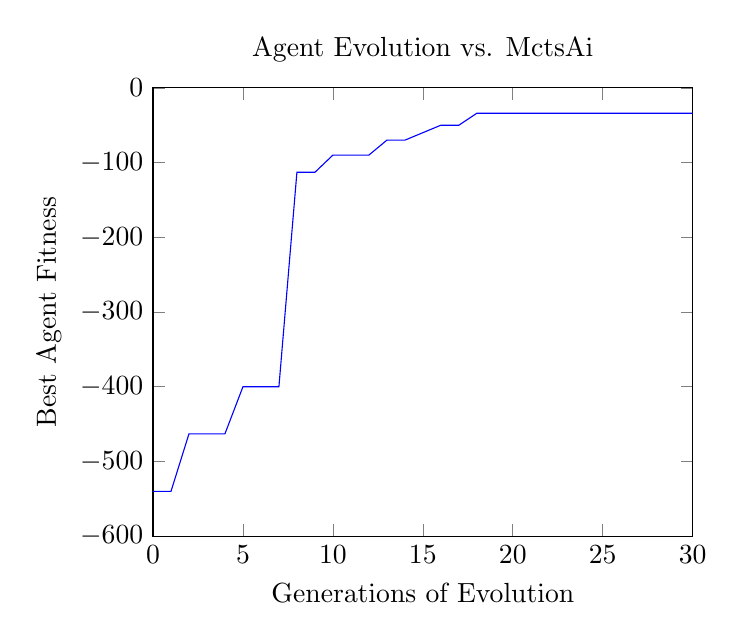
\begin{tikzpicture}
\begin{axis}[
align=center,
title={Agent Evolution vs. MctsAi},
xlabel={Generations of Evolution},
ylabel={Best Agent Fitness},
xmin=0, xmax=30,
ymin=-600, ymax=0,
xtick={0,5,10,15,20,25,30},
ytick={-600,-500,-400,-300,-200,-100,0},
]
\addplot[
color=blue
]
coordinates {
	(0,-540)
	(1,-540)
	(2,-463)		
	(3,-463)
	(4,-463)
	(5,-400)
	(6,-400)
	(7,-400)
	(8,-113)
	(9,-113)
	(10,-90)
	(11,-90)
	(12,-90)
	(13,-70)
	(14,-70)
	(15,-60)
	(16,-50)
	(17,-50)
	(18,-34)
	(19,-34)
	(20,-34)
	(21,-34)
	(22,-34)
	(23,-34)
	(24,-34)
	(25,-34)
	(26,-34)
	(27,-34)
	(28,-34)
	(29,-34)
	(30,-34)
};
\end{axis}
\end{tikzpicture}
\end{center}
\caption{Plot of the agent's evolution vs. the MctsAi. Agent's fitness on the y-axis and number of generations on the x.}
\end{figure}
\newpage
The agent exhibited some unusual behaviours during its evolution, which are interesting since they would not have necessarily be thought of during the design stage. One interesting behaviour the agent showed was a strategy of attacking the opponent, jumping over the opponent's head, and then attacking from the opposite side. The behaviour resulted in a high fitness and occurred frequently during the evolution, possibly due to the fact that the agent becomes more difficult to attack while moving constantly. Another interesting behaviour was the agent going to the edge of the game arena and constantly crouching to avoid enemy attacks. This was generally lost during the evolution stage due to the overly defensive playstyle of the agent. A final behaviour exhibited is the constant use of attacks by the agent. Even while stationary, the speed in which the agent can use attacks is relatively fast and often appears as a solution to the problem in later generations.\\ 

One problem encountered during the agent evolution was the presence of a noisy environment. The environment of the game is quite complex and dynamically changing, the agent's performance is heavily based on the performance of its opponent. The presence of this noisy environment meant that some genotypes did not result in a similar expected fitness when evolved with genetic operators. To tackle this problem we introduced the notion of elitism to our algorithm, causing the best genotypes of a generation to be kept regardless. We also improved our genetic operators to operate more effectively based on their application to an artificial neural network. Agent evolution in a static game, such as Mario, would likely see a smoother learning rate.\\

From the introduction of an incremental learning environment in the next prototype, we hope to see an improvement in the agent's rate of evolution. Providing incrementally more complex tasks will hopefully allow our agent to formalise a suitable strategy quickly which is applicable to all opponents in the game. We will also assess whether the incremental environment will improve our agent's learning capabilities to the point of beating other AI such as the MctsAi agent.\\


\newpage
\subsection{Prototype Three: Appropriate Learning Method Implemented in Incremental Evolution Environment}
Due to the complex behaviour our agent must exhibit and the noisy environment it is being implemented in, the use of an incremental evolution environment may be beneficial. In an incremental evolution environment, the agent is faced with increasingly complex challenges in hope that it will improve the agent's rate of evolution. The agent's evolution will be assessed by comparing it to that of another agent who does not utilise the incremental environment.\\
\newpage
\subsubsection{Design}
For our incremental evolution environment we will use three stages of complexity for the agent to compete versus. We will attempt to create a gradual increase in complexity for the tasks to allow our agent to quickly evolve applicable behaviours. From this use of an incremental environment we will then be able to evaluate whether the environment improves the agent's rate of evolution, and therefore assess the validity of hypothesis H1.\\

The first stage of incremental evolution, referred to as INC0, was an agent who did not move. Since the agent was not needed to output any actions or process any game data, there was no design needed. All the agent needed to accomplish was to be functional in the game framework. We expect the evolution of this stage for the learning agent to be relatively fast since the opponent is stationary. A stationary opponent causes no threat as they will not attack back and will not attempt to evade incoming attacks. During this stage of incremental evolution the learning agent should be able to learn how to maximise its damage dealt.\\

The next stage of incremental evolution (INC1) was an opponent who moves in random directions though does not attack. This was seen to be an incremental step up in complexity from the previous stage, INC0, since the opponent will still be able to attack back though will now have the ability to potentially evade agent attacks. The implementation of this incremental stage will involve the agent selecting movement directions based on the result of a randomly generated value.\\

For the final incremental stage (INC2) the tasks complexity was increased by allowing the opponent agent to both move and attack randomly. Compared to the other steps of incremental evolution, this was quite a large jump in complexity since the agent can now be damaged. This means that the agent can no longer mindlessly attack its opponent and now must take its opponents actions into consideration. The stage will be implemented similarly to the RandomAi agent from the FightingICE website.\\
\newpage
\subsubsection{Implementation}
\subsubsection*{Incremental Stage 0 - INC0}
For the initial stage of incremental evolution we decided to use an agent who does not move at all as the evolving agent's opponent. All that is needed for the agent is for it to function in the FightingICE game framework.\\

In order to be implemented in the FightingICE framework, the agent's controller class implements the AIInterface Java interface. Since the agent will be stationary, no processing or extra code was needed except for the agent's initialisation. Agent initialisation was as normal: initialising the CommandCenter and FrameData object as well as a Key object. The character being played (in this case CHARACTER\_ZEN), also needed to be declared in the getCharacter method to ensure agent functionality.

\subsubsection*{Incremental Stage 1 - INC1}
For the next incremental stage of evolution we used an agent who moves randomly, though does not attack. In order to implement this agent, the controller's class, inc1.java, implements the AIInterface interface. To output random movement actions with the agent we used a Java Random object which is initialised in the interface's initialize method.\\

To generate the random movement action the nextInt method from the Random object is called with an argument of 4, corresponding to each direction of movement (up, down, left, right). A switch case in then used to determine which of the agent's actions are output based on the value of the randomly generated value. Code for the stage's switch case is shown in listing 15.

\singlespacing
\begin{lstlisting}[caption=INC1 switch case.]
int action = rnd.nextInt(4);
switch (action) {
	case 0:
		inputKey.D = true;
		break;
	case 1:
		inputKey.R = true;
		break;
	case 2:
		inputKey.L = true;
		break;
	case 3:
		inputKey.U = true;
		break;
}
\end{lstlisting}
\newpage

\onehalfspace
\subsubsection*{Incremental Stage 2 - INC2}
For the final stage of incrementally increasing complexity, we decided to use an opponent agent who moves and attacks randomly. The agent was implemented similarly to the RandomAI agent provided on the FightingICE website.\\

In order to output actions at random, this stage had to make use of a Java Random object. This object would be used to which random action the agent outputs. The Random object is initialised through the initialize method, called when the agent is initialised. The class also initialises a Key object so that the agent can output actions to the framework. To determine which action is output, a boolean expression is used to check whether the next integer value generated between 1 and 10 is greater than 5. If the boolean value is true then the action is output, else it is not and the next action is evaluated. This results in each action having a 50\% chance of being output by the agent. An excerpt of the code showcasing the random selection of actions is seen in listing 16.\\

\singlespacing
\begin{lstlisting}[caption=INC2 random action selection.]
@Override
public void processing() {
	// Choose next action at random
	inputKey.A = (rnd.nextInt(10) > 4) ? true : false;
	inputKey.B = (rnd.nextInt(10) > 4) ? true : false;
	inputKey.C = (rnd.nextInt(10) > 4) ? true : false;
	inputKey.U = (rnd.nextInt(10) > 4) ? true : false;
	inputKey.D = (rnd.nextInt(10) > 4) ? true : false;
	inputKey.L = (rnd.nextInt(10) > 4) ? true : false;
	inputKey.R = (rnd.nextInt(10) > 4) ? true : false;
}	
\end{lstlisting}

\newpage
\onehalfspace
\subsubsection{Evaluation}
The first stage of incremental learning to evaluate was INC0. In INC0, the agent is stationary and does not move or attack. Due to the relatively simple nature of this task, we expect the agent to evolve to its maximum potential relatively quickly. We will then be able to apply the next incremental stage to the agent to determine whether the incremental learning approach is effective. Each incremental stage will be run with the same genetic algorithm parameters as that of prototype 2.\\

The graph shown in figure 9 is a plot showing the agent's improvement after generations of evolution. For the initial 5 generations, the agent is unable to find a solution to improve its fitness, dealing around 100 damage to the opponent. This initial plateau may be due to a lack of diversity within our genetic operators, or an inappropriately small population size. The agent then sees irregular though consistent improvements in its performance up until around 20 generations. After generation 20, the agent's performance plateaus at a fitness of 1140. This fitness represents the capability of the agent at the current stage as extensive evolution beyond this has no effect on the agent's performance. \\

\begin{figure}[h]
\begin{center}
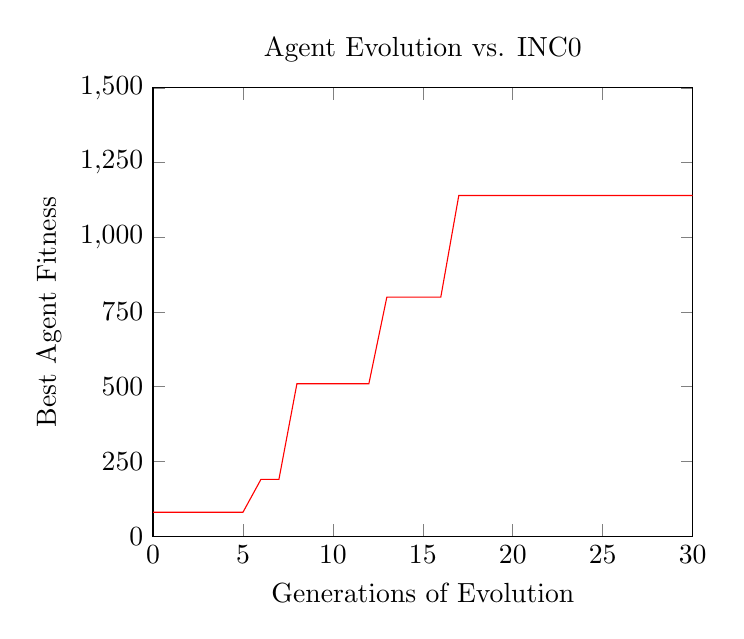
\begin{tikzpicture}
\begin{axis}[
align=center,
title={Agent Evolution vs. INC0},
xlabel={Generations of Evolution},
ylabel={Best Agent Fitness},
xmin=0, xmax=30,
ymin=0, ymax=1500,
xtick={0,5,10,15,20,25,30},
ytick={0,250,500,750,1000,1250,1500},
]
\addplot[
color=red
]
coordinates {
	(0,80)
	(1,80)
	(2,80)		
	(3,80)
	(4,80)
	(5,80)
	(6,190)
	(7,190)
	(8,510)
	(9,510)
	(10,510)
	(11,510)
	(12,510)
	(13,800)
	(14,800)
	(15,800)
	(16,800)
	(17,1140)
	(18,1140)
	(19,1140)
	(20,1140)
	(21,1140)
	(22,1140)
	(23,1140)
	(24,1140)
	(25,1140)
	(26,1140)
	(27,1140)
	(28,1140)
	(29,1140)
	(30,1140)
};
\end{axis}
\end{tikzpicture}
\caption{Plot of the agent's fitness over generations when competing versus the first stage of incremental evolution (INC0).}
\end{center}
\end{figure}
\newpage
During the evolution some unusual behaviour emerged from the agent. One being that exhibited in prototype 2, where the agent's strategy is to attack the opponent, jump over its head and then attacking from the opposite side. This strategy proved effective for this stage of evolution due to the in-game physics. Attacking a character multiple times from the same direction causes the characters body to be pushed away, until eventually both players are at the edge of the arena. When utilising this jumping strategy, the agent is able to keep the opponent's character in a single position, easing the damage dealing process. Other behaviours exhibited include the agent walking up to the opponent and constantly pressing an attack button.\\

Next we evaluated the agent's performance versus the next stage of incremental evolution- INC1, displayed in figure 10. For this stage, the agent's opponent was an agent who moved randomly, though did not use any of the in-game attacks. This was seen to be an incremental step up in complexity from the initial agent who does not move at all. The initial population used for the evolution was the final population from the evolution against INC0. This was in hope that the performance learned by the agent in the initial incremental stage will be transferable and applicable for this stage, too.\\

\begin{figure}[h]
\begin{center}
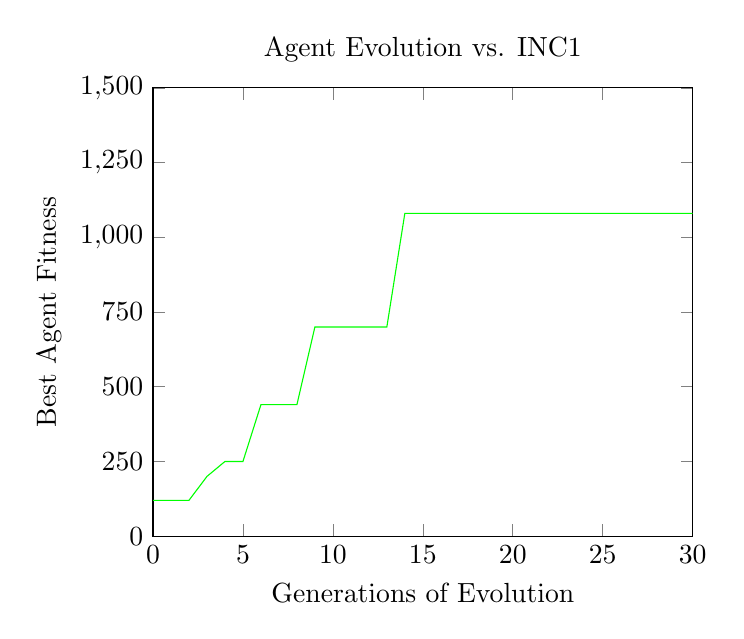
\begin{tikzpicture}
\begin{axis}[
align=center,
title={Agent Evolution vs. INC1},
xlabel={Generations of Evolution},
ylabel={Best Agent Fitness},
xmin=0, xmax=30,
ymin=0, ymax=1500,
xtick={0,5,10,15,20,25,30},
ytick={0,250,500,750,1000,1250,1500},
]
\addplot[
color=green
]
coordinates {
	(0,120)
	(1,120)
	(2,120)		
	(3,200)
	(4,250)
	(5,250)
	(6,440)
	(7,440)
	(8,440)
	(9,700)
	(10,700)
	(11,700)
	(12,700)
	(13,700)
	(14,1080)
	(15,1080)
	(16,1080)
	(17,1080)
	(18,1080)
	(19,1080)
	(20,1080)
	(21,1080)
	(22,1080)
	(23,1080)
	(24,1080)
	(25,1080)
	(26,1080)
	(27,1080)
	(28,1080)
	(29,1080)
	(30,1080)
};
\end{axis}
\end{tikzpicture}
\caption{Plot of the agent's performance against generations when fighting versus the INC1 incremental evolution stage.}
\end{center}
\end{figure}
\newpage
A positive change is seen in the initial (0th) generations fitness, although only minor. It is difficult whether to say this evolutionary improvement is related to introduction of incremental learning or whether it was just a lucky result in a near-random search. From here, the agent's performance increases over generations, until it hits a plateau at a similar point to INC0. This stage of incremental learning hits the plateau earlier, at around generation 15: instead of 18 as it was in INC0. At this stage it is difficult to assess whether the incremental environment has been implemented successfully. Instead, we aim to evaluate the evolution rate of an agent not using the environment to that of one that does.\\ 

Following this, we evaluated the agent's performance versus the final incremental stage, INC2, shown in figure 11. This stage incrementally increases the task complexity by now allowing the opponent to both move and attack, instead of only movement. Since the opponent is now attacking the agent, it may make the evolution process more difficult. Strategies which focused on sheer damage to the enemy over defence may now be redundant. The evolution for this stage began with the initial generation being the final of INC1's evolution.\\

\begin{figure}[h]
\begin{center}
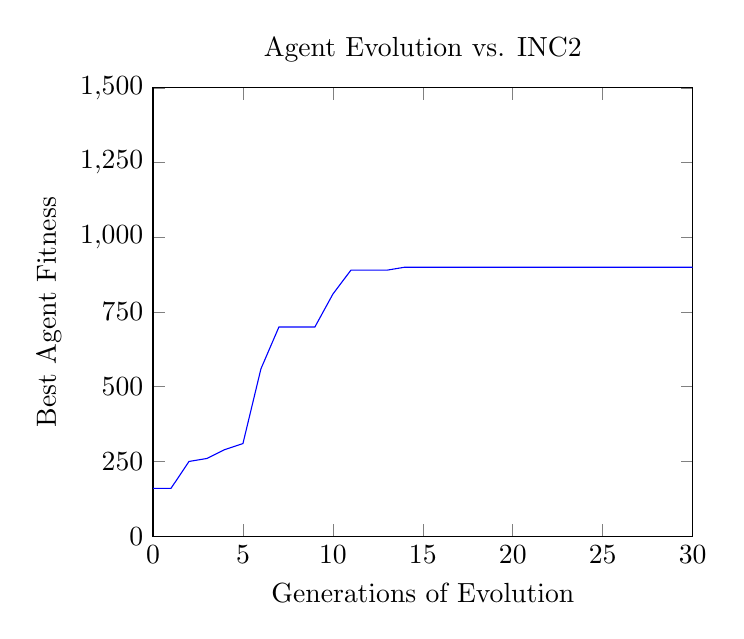
\begin{tikzpicture}
\begin{axis}[
align=center,
title={Agent Evolution vs. INC2},
xlabel={Generations of Evolution},
ylabel={Best Agent Fitness},
xmin=0, xmax=30,
ymin=0, ymax=1500,
xtick={0,5,10,15,20,25,30},
ytick={0,250,500,750,1000,1250,1500},
]
\addplot[
color=blue
]
coordinates {
	(0,160)
	(1,160)
	(2,250)		
	(3,260)
	(4,290)
	(5,310)
	(6,560)
	(7,700)
	(8,700)
	(9,700)
	(10,810)
	(11,890)
	(12,890)
	(13,890)
	(14,900)
	(15,900)
	(16,900)
	(17,900)
	(18,900)
	(19,900)
	(20,900)
	(21,900)
	(22,900)
	(23,900)
	(24,900)
	(25,900)
	(26,900)
	(27,900)
	(28,900)
	(29,900)
	(30,900)
};
\end{axis}
\end{tikzpicture}
\caption{Agent's performance over evolution versus the final INC2 incremental learning stage.}
\end{center}
\end{figure}
\newpage
The agent's fitness began as a positive value, meaning that the fittest agent manages to beat the random action AI over three rounds. This demonstrates the effectiveness of the incremental environment, with the agent initially being able to win versus an attacking opponent without any generations of evolution. The agent's fitness then rises steadily until around generation 10 where it plateaus at 900 fitness. Due to the opponent now being able to attack, the highest potential fitness of the agent was released (other incremental stages saw fitness of 1000+). This ability for the opponent to attack also creates a more noisy environment, where genotypes with high fitness do not necessarily achieve the same results when run a second time. The fitness within these generations was usually well spread, with some individuals having a very high fitness and others with little or none. This showcases the genetic diversity of the method and the variety of solutions being evaluated.\\

Finally, we needed to assess the impact the implementation of the incremental learning environment had on the rate of evolution for the agent. This assessment will allow us to determine the truth of hypothesis H1- the incremental learning environment will have a positive effect on the agent's evolution rate. We can prove this truth by presenting the evolution rate of an agent using an incremental learning environment and one without, and comparing the results of the two. If the agent implementing incremental learning sees a faster evolution we can determine the hypothesis to be true.\\

In order to assess the effectiveness of the incremental environment we ran two evolutions. Both agents were fighting versus the MctsAi agent, although only one of the agents implemented an incremental learning environment. In order to improve itself with the incremental environment, the agent must first train itself on these less complex tasks. Once the evolution of the final incremental stage is complete, the final generation of that evolution is pipelined into the MctsAi agent evolution. This allows the agent to develop some understanding of the game and develop strategies before the evolution begins, giving it a head-start over other agents.\\
\newpage
The plot for this comparison is shown in figure 12. The blue plot represents the evolution of a neuroevolution agent which does NOT utilise an incremental learning environment whereas the red represents an agent which does. The graph shows the incremental agent reaching a much higher fitness in the initial generation due to the pre-training from incremental tasks. After around 10 generations of evolution, the incremental agent hits a plateau of a similar fitness to that of the agent not using incremental learning. This plateau is known as the skill ceiling of the agent, where improvements would only be seen by adding agent capabilities or adapting the information received by it. However, the incremental agent hits this skill ceiling much earlier than its counterpart, showcasing the effect of incremental learning environments.\\

\begin{figure}[h]
\begin{center}
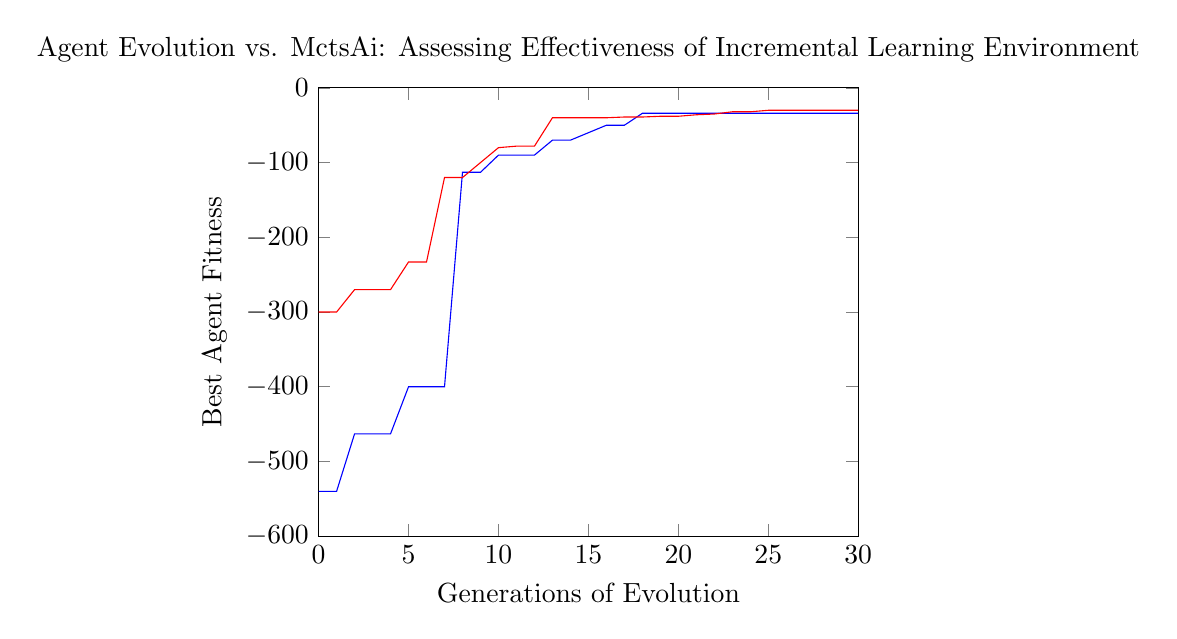
\begin{tikzpicture}
\begin{axis}[
align=center,
title={Agent Evolution vs. MctsAi: Assessing Effectiveness of Incremental Learning Environment},
xlabel={Generations of Evolution},
ylabel={Best Agent Fitness},
xmin=0, xmax=30,
ymin=-600, ymax=0,
xtick={0,5,10,15,20,25,30},
ytick={-600,-500,-400,-300,-200,-100,0},
]
\addplot[
color=blue
]
coordinates {
	(0,-540)
	(1,-540)
	(2,-463)		
	(3,-463)
	(4,-463)
	(5,-400)
	(6,-400)
	(7,-400)
	(8,-113)
	(9,-113)
	(10,-90)
	(11,-90)
	(12,-90)
	(13,-70)
	(14,-70)
	(15,-60)
	(16,-50)
	(17,-50)
	(18,-34)
	(19,-34)
	(20,-34)
	(21,-34)
	(22,-34)
	(23,-34)
	(24,-34)
	(25,-34)
	(26,-34)
	(27,-34)
	(28,-34)
	(29,-34)
	(30,-34)
};
\addplot[
color=red
]
coordinates {
	(0,-300)
	(1,-300)
	(2,-270)		
	(3,-270)
	(4,-270)
	(5,-233)
	(6,-233)
	(7,-120)
	(8,-120)
	(9,-100)
	(10,-80)
	(11,-78)
	(12,-78)
	(13,-40)
	(14,-40)
	(15,-40)
	(16,-40)
	(17,-39)
	(18,-39)
	(19,-38)
	(20,-38)
	(21,-36)
	(22,-35)
	(23,-32)
	(24,-32)
	(25,-30)
	(26,-30)
	(27,-30)
	(28,-30)
	(29,-30)
	(30,-30)
};
\end{axis}
\end{tikzpicture}
\end{center}
\caption{Two plots of the agent's evolution versus the MctsAi agent. Blue plot represents agent who has been evolved without the use of an incremental learning environment. Red plot implements this incremental environment and evolves on before evolution.}
\end{figure}

From this evolution data, we can assess the validity of hypothesis H1: the agent's evolution will benefit from incrementally more complex scenarios. From comparing the two plots, we see an obvious speed improvement in the agent's evolution. Even from the initial generation, the incrementally trained agent has a fitness which is not reached until the 8th or 9th generation of its counterpart. The incremental learning environment also causes the agent to hit its skill ceiling / plateau faster. From this, we can decude that H1 is true and the agent will benefit from an incremental learning environment. However, we should also consider whether the time taken to evolve agents capable of completing these incremental tasks outweighs that of simply evolving the agent repeatedly.\\

\newpage
\section{Testing and Performance Assessment}
For the testing of our agent and to assess its performance, we decided to evaluate three separate agents from different stages of evolution. These agent's were hand selected from the evolution data and were desired to be of easy, moderate, and difficult levels of difficulty. \\

The first agent to be tested was to be an agent of easy difficulty. The agent was chosen from an early generation of evolution and was therefore less competitive than its counterparts. The agent jumped often, attempting to execute the strategy seen in the prototype evolution of kicking the opponent, jumping over its head, then kicking from the opposite side. However, since this agent was selected from an early stage of evolution the kicks were mistimed and misplaced which made them easily countered.\\

The next agent to be evaluated is that of what was considered moderate difficulty and chosen from a point mid-way through evolution. This agent mostly stayed on the ground, preferring to traverse the arena via movement to the left and right, though acts very aggressively. The agent's strategy is to achieve the perfect distance between the characters in order to attack with a high aimed kick. This strategy proves effective since the high aimed kick has a long range and is difficult to counter.\\

The final agent to be evaluated was rated difficult. This agent, likewise to the easy, jumped often and attempts to kick its opponent from the air. However due to the later stage of evolution, the agent's actions are more refined and difficult to counter. The consistent air movement also makes the agent's movements difficult to predict, making it harder for the opponent to successfully hit the opponent. The agent's strategies are mostly aggressive however there is a deadlock situation that can occur where the agent repeatedly crouches. The agent does so defensively and once the opponent nears the agent will usually kick or use an appropriate attack for the situation at hand.

\newpage
Results for each agent's performance against a human opponent are displayed in the table of figure 13. The agent's performance is calculated through: the agents hit-points at the end of the round - the human opponent's hit-points at the end of the round. The last column is used to average results from the 3 rounds and determine the agent's overall performance.\\

\begin{figure}[h]
\begin{tabular}{|p{0.3\linewidth}|p{0.1\linewidth}|p{0.1\linewidth}|p{0.1\linewidth}|p{0.2\linewidth}|}
\hline
Agent Difficulty & Round 1 Result & Round 2 Result & Round 3 Result & Average Performance\\ \hline
Easy & -160 & -234 & -215 & -169\\ \hline
Moderate & 147 & -26 & 37 & 52\\ \hline
Difficult & 168 & 145 & 250 & 187\\ \hline
\end{tabular}
\caption{Table showing different difficulty level agents results versus a human opponent.}
\end{figure}

\vspace{8mm}

When the easy agent was played the agent lost every round, with an average performance of -169. This means that the agent had on average 169 less hit-points than the human opponent at the end of every round. The moderate agent saw better results, winning two of the three rounds and receiving an average performance of 52 health advantage per round. When facing the difficult agent, the human opponent was unable to win any rounds, with the agent comfortably winning consistently.\\

From these results we can assess the validity of hypothesis H2- neuroevolution will evolve an agent to the point of being competitive versus a human to be true. The agent's performance is displayed in both moderate and difficult difficulties, where the human opponent struggles to win a single round. This demonstrates the competitive challenge an evolved agent can provide a human. In order to select an agent of an appropriate skill level to be competitive versus the opponent, the agent should be picked based on its current stage of evolution. Agent in early stages of evolution picked for new human players and heavily evolved agents for the more experienced players. This work could also be extended by the agent storing the network weights for each of these difficulties and adapting the difficulty chosen / its playstyle based on the opponent's skill.\\

To view the agent's performance against a human opponent please see the following links:
\begin{itemize}
\item {Easy agent - https://youtu.be/HYh8m1mTIg4}
\item {Moderate agent - https://youtu.be/EIxX\_CfB4Q0}
\item {Difficult agent - https://youtu.be/Zam8Sm1cCwM}
\end{itemize}
\newpage
\section{Conclusions}

In this section of the dissertation we will conclude our findings from the work. To do this we will assess whether our hypotheses were found to be true and comment on other relevant thoughts and findings. From this we hope to evaluate the meaning of our results and present them in a formal fashion. The main achievements of the dissertation will be provided along with the main limitations and any possible extensions or future work.\\

To remind ourselves, the project hypotheses were as follows: 
\begin{itemize}
\item {H1: The agent's evolution will benefit from the introduction of incrementally more complex scenarios.}
\item {H2: Neuroevolution will be able to evolve the agent to a stage of being competitive versus a human opponent.}
\end{itemize}

To assess whether the first hypothesis was proven, we consult the Evaluation section of prototype 3. From the evolution data of one agent without the use of incremental learning and one with, we saw that the agent utilising the incremental technique resulted in an improved starting fitness of the agent. Therefore we can determine the hypothesis to be proven true. However, the main issue with using an incremental learning method is whether the time spent evolving the agent through incrementally more complex challenges outweighs the time it would spend evolving without the incremental environment. The overall evolution process was eased by the introduction of incremental challenges, though it would maybe have been more suitable to measure the time taken to reach a certain fitness with or without the use of an incremental environment.\\

The second hypothesis was to determine whether neuroevolution could be used to evolve the agent to a competitive stage. This was assessed during section 5 of the dissertation, Testing and Performance Assessment. This hypothesis is seen to be proved, since the agents were clearly competitive opponents for the human player. Agents of both moderate and difficult difficulty were able to beat the human opponent, with the difficult agent winning all three rounds. Obviously this is also a subjective statement, since an agent who is competitive versus one human opponent is not necessarily competitive against another human of higher skill. We were not able to implement an agent which updates its play-style based on the current game state since it would involve adapting the network weights during run-time, whereas we want training to be the method of weight optimisation.\\
\newpage
The main achievements of this dissertation include the fact that neuroevolution was successfully implemented and evolution saw an increase in agent's fitness. The main goal of this dissertation was the implementation of neuroevolution in order to evaluate its effectiveness, therefore having a working implementation is essential. Another achievement is the fact that both hypotheses were able to be proven. Proving the hypotheses is the goal of this application and the correct implementation of the agent and its environment allowed us to achieve this. The performance capability of the agent is also an achievement which can be seen. At harder difficulty levels, the agent is able to consistently win versus a human opponent, as seen in section 5 (Testing and Performance Assessment). The agent also performs reasonably well versus other intelligent agents provided on the FightingICE website.\\

The limitations of this dissertation include the fact that the agent was not able to evolve past the point of beating other agents provided from the FightingICE website. Evolving the agent against the MctsAi, even after using an incremental environment, resulted in agents close to but unable to beat the opponent. Improving our agent by either providing it more information through increasing the number of inputs to the neural network, or applying more parameter tuning to the network may allow our agent to beat opposing agents. Another limitation with the dissertation was the jump during incremental evolution. Going from a random action agent to an advanced one such as MctsAi is a huge jump in task complexity. By providing smaller incremental steps in complexity, we may have been able to evolve our agent to a higher performance level.\\

From this work there is further work which could potentially be implemented in the FightingICE framework. Improvements could be made to this dissertation's agent to see if improvement in performance can be seen. Many improvements could be made to the agent such as increasing the number of inputs to the agent's network: this could also involve visual RGB data to receive information without delay. More work could also be done in optimising parameters for the agent and its evolution. From these optimisations we could find suitable genetic algorithm parameters and determine whether the neural network is complex enough or the need for more layers / deep learning is required.\\
\newpage
Further work could also be done into implementing other types of agents in the FightingICE game framework. Due to the now-familiarity with the framework, we could look into implementing more advanced agents utilising alternate machine learning methods, such as an extensive rule based agent. We could also compare these newly implemented agents to the agent of this dissertation, and evaluate the effectiveness of learning which is produced.\\

A final area of further work is work outside of the FightingICE framework but using artificial intelligence methods. This could include Starcraft's DeepMind framework when it is released, where other AI methods such as swarm robotics can be implemented. Agents outside of games can also be considered too, for example in other simulators. One interesting environment to implement these agents would be in a water based simulation scenario.

\singlespacing
\newpage
\section{References}
\begin{thebibliography}{10}

\bibitem{michalski}
	Michalski, R., Carbonell, J. and Mitchell, T.
	(1983).
	Machine Learning: An Artificial Intelligence Approach. 
	pp. 5-20.
	

\bibitem{nnm}
	Wilde, P.
	(1997).
	Neural Network Models.
	[book]
	pp. 4-14.
	
\bibitem{reinforce}
	Barto, S. and Sutton R.
	(1998).
	Reinforcement Learning: An Introduction.
	pp. 23-30.
	
\bibitem{search}
	McCallum, A., Nigam, K., Rennie, J. and Seymore, K.
	(2001).
	A Machine Learning Approach to Building Domain-Specific Search Engines.
	[online]
	Available at: http://www.kamalnigam.com/papers/cora-ijcai99.pdf
	[Accessed 23 Nov. 2016]
	
\bibitem{ocr}
	Wernick, M., Yang, Y. and Strother, S.
	(2010).
	Machine Learning in Medical Imaging.
	[online]
	Available at: https://www.ncbi.nlm.nih.gov/pmc/articles/PMC4220564/
	[Accessed 23 Nov. 2016]
	
\bibitem{ea}
	Prins, C.
	(2004).
	A simple and effective evolutionary algorithm for the vehicle routing problem.
	[book]
	pp. 20-35.	

\bibitem{neapps}
	Neural Networks Research Group
	(2014).
	Research on Neuroevolution Applications.
	[online]
	Available at: http://www.cs.utexas.edu/users/nn/pages/research/ne-applications.html
	[Accessed 23 Nov. 2016]
	
\bibitem{fightingice}
	Intelligent Computer Entertainment Lab, Ritsumeikan University.
	(2010).
	FightingGameAICompetition.
	[online]
	Available at: http://www.ice.ci.ritsumei.ac.jp/~ftgaic/
	[Accessed 23 Nov. 2016]

\bibitem{risi}
	Risi, S. and Togelius, J.
	(2015).
	Neuroevolution in Games: State of the Art and Open Challenges.
  	[online]
  	Available at: https://arxiv.org/pdf/1410.7326.pdf
  	[Accessed 03 Nov. 2016]

\bibitem{pace}
	Pace, A.
	(2014).
	Improving AI for simulated cars using Neuroevolution.
	[online]
	Available at: http://commerce3.derby.ac.uk/ojs/index.php/gb/article/view/3/1
	[Accessed 07 Nov. 2016]
	
\bibitem{lampro}
	Lampropoulos, A.
	(2005).
	Machine Learning Paradigms.
	[online]
	Available at: http://file.allitebooks.com/20150722/Machine\%20Learning\%20Para-digms-\%20Applications\%20in\%20Recommender\%20Systems.pdf
	[Accessed 18 Nov. 2016]
  
\bibitem{incre}
	Gomez, F. and Miikkulainen, R.
	(1997).
	Incremental Evolution of Complex General Behaviour
	[online]
	Available at: http://nn.cs.utexas.edu/downloads/papers/gomez.adaptive-behavior.pdf
	[Accessed 18 Nov. 2016]
	
\bibitem{dota}
	Batsford, T.
	(2014).
	Calculating Optimal Jungling Routes in DOTA2 Using Neural Networks and Genetic Algorithms.
	[online]
	Available at: http://commerce3.derby.ac.uk/ojs/index.php/gb/article/view/14/12
	[Accessed 18 Nov. 2016]
	
\bibitem{atari}
	Hausknecht, M., Lehman, J. and Stone, P.
	(2014).
	A Neuroevolution Approach to General Atari Game Playing.
	[online]
	Available at: https://www.cs.utexas.edu/~mhauskn/papers/atari.pdf
	[Accessed 15 Nov. 2016]
	
\bibitem{genvid}
	Braylan, A., Hollenbeck, M., Meyerson, E. and Miikkulainen, R.
	(2015).
	Reuse of Neural Modules for General Video Game Playing
	[online]
	Available at: https://arxiv.org/pdf/1512.01537v1.pdf
	[Accessed 17 Nov. 2016]
	
\bibitem{swarmann}
	Dehuri, S., Ghosh, S., and Cho, S-B
	(2011).
	Integration of Swarm Intelligence and Artificial Neural Network.
	[book]
	P1-P23

\bibitem{percept}
	Widrow, B. and Lehr, A.
	(1990).
	30 Years of Adaptive Neural Networks: Perceptron, Madaline, and Backpropagation.
	[online]
	Available at: https://pdfs.semanticscholar.org/8b73/adda1-5fa71b0a35ffedb899d6a72d621923b.pdf
	[Accessed 24 Nov. 2016]
	
\bibitem{ffann}
	Hornik, K.
	(1989).
	Multilayer Feedforward Networks are Universal Approximators.
	[online]
	Available at: http://deeplearning.cs.cmu.edu/pdfs/Kornick\_et\_al.pdf
	[Accessed 24 Nov. 2016]
	
\bibitem{nnapps}
	Stanford University.
	(2013).
	Applications of neural networks.
	[online]
	Available at: http://cs.stanford.edu/people/eroberts/courses/soco/projects/neural-networks/Applications/index.html
	[Accessed 24 Nov. 2016]
	
\bibitem{activate}
	Hornik, K.
	(1990).
	Approximation Capabilities of Multilayer Feedforward Networks.
	[online]
	Available at: http://zmjones.com/static/statistical-learning/hornik-nn-1991.pdf
	[Accessed 24 Nov. 2016]
	
\bibitem{gas}
	Vavak, F. and Fogarty, T.
	(1996).
	Comparison of Steady State and Generational Genetic Algorithms for Use in Nonstationary Environments.
	[online]
	Available at: http://citeseerx.ist.psu.edu/viewdoc/download?doi=10.1.1.55.3585-\&rep=rep1\&type=pdf
	[Accessed 24 Nov. 2016]
	
\bibitem{neat}
	Kenneth, S. and Miikkulainen, R.
	(2002).
	Evolving neural networks through augmenting topologies.
	[book]
	pp. 1-30.
	
\bibitem{hyperneat}
	Kenneth, S., D'Ambrosio, D. and Gauci, J.
	(2009).
	A hypercube-based encoding for evolving large-scale neural networks.
	[book]
	pp. 05-09.
	
\bibitem{hypehype}
	Evolutionary Complexity Research Group at UCF.
	(2003).
	The hypercube-based neuroevolution of augmenting topologies (HyperNEAT).
	[online]
	Available at: http://eplex.cs.ucf.edu/hyperNEATpage/
	[Accessed 24 Nov. 2016]
\end{thebibliography}
\newpage
\section{Appendices}
\subsection*{Figure 1}
Multi-layer feed forward artificial neural network.	\\
https://static1.squarespace.com/static/51d342a0e4b0290bcc56387d/t\\ /54497f24e4b0c5079a9976ef/1414102821758/
\subsection*{Figure 2}
Hyperbolic tangent function plot.\\
http://www.mpe.mpg.de/~ott/dpuser/tanh.png
\subsection*{Figure 3}
Example of genotype representation.\\
Self-made
\subsection*{Figure 4}
Illustration of two-point crossover.\\
http://www.stumptown.com/diss/gacross.jpg
\subsection*{Figure 5}
Image of a biological neuron\\
https://online.science.psu.edu/sites/default/files/bisc004/content/neuron.jpg
\subsection*{Figure 6}
Screenshot of the FightingICE game platform.\\
http://www.stumptown.com/diss/gacross.jpg
\subsection*{Figure 7}
Labelled inputs taken by ANN.\\
Self-made- annotated screenshot
\newpage
\subsection{Prototype 1}
\subsubsection{Prototype1.java}
\begin{lstlisting}
import commandcenter.CommandCenter;
import enumerate.Action;
import java.lang.Math;
import java.util.Arrays;

import structs.FrameData;
import structs.GameData;
import structs.Key;
import structs.MotionData;
import gameInterface.AIInterface;


public class Prototype1 implements AIInterface {
	ANN ann;
	boolean p;
	GameData gd;
	Key inputKey;
	FrameData fd;
	CommandCenter cc;
	
	@Override
	public int initialize(GameData gameData, boolean playerNumber) {
		// TODO Auto-generated method stub
		gd = gameData;
		p = playerNumber;
		inputKey = new Key();
		fd = new FrameData();
		cc = new CommandCenter();
		ann = new ANN();
		return 0;
	}

	@Override
	public void getInformation(FrameData frameData) {
		// TODO Auto-generated method stub
		fd = frameData;
		cc.setFrameData(fd, p);

	}

	@Override
	public void processing() {
		if(!fd.getEmptyFlag()){
			if(fd.getRemainingTime() > 0){	
				//System.out.println(cc.getEnemyX());
				// X RANGE -120 530
				//System.out.println(cc.getEnemyY());
				// feeds through network
				double[] out = ann.feed(
					Math.tanh((double)cc.getMyX()),			// horizontal distance
					Math.tanh((double)cc.getMyY()),			// vertical distance
					Math.tanh((double)cc.getMyEnergy())		// player's energy
				);
				inputKey.A = (out[0] > 0) ? true : false;
				inputKey.B = (out[1] > 0) ? true : false;
				inputKey.C = (out[2] > 0) ? true : false;
				inputKey.U = (out[3] > 0) ? true : false;
				inputKey.D = (out[4] > 0) ? true : false;
				inputKey.L = (out[5] > 0) ? true : false;
				inputKey.R = (out[6] > 0) ? true : false;
			}
		}
	}

	@Override
	public Key input() {
		// TODO Auto-generated method stub
		return inputKey;
	}

	@Override
	public void close() {
		// TODO Auto-generated method stub

	}

	public String getCharacter(){
		return CHARACTER_ZEN;
	}

}

\end{lstlisting}
\newpage
\subsubsection{ANN.java}
\begin{lstlisting}
import java.util.Random;
import structs.Key;
/**
 * Implements a 3-layer artificial neural network with 3 input
 * nodes, 10 hidden layer nodes and 7 output nodes. Output nodes
 * refer to the 7 possible key presses; input nodes are defaultly
 * horizontal distance, vertical distance and player energy.
 * 
 * @author Robbie Dunn
 *
 */
public class ANN {
  
  private double[][] weights0;    // weights for 0th network layer
  private double[][] weights1;    // weights for 1st network layer

  /* declares and initialises weights randomly (-1.0, 1.0) */
  public ANN() {
    weights0 = new double[3][10];
    weights1 = new double[10][7];
    Random rand = new Random();
    
    // initialising weights
    for(int i=0;i<10;i++) {   // for each hidden layer node
      for(int j=0;j<3;j++) {  // for each input layer node
        weights0[j][i] = (rand.nextDouble() * 2) - 1; // weight initiailised between -1/1
      }
      for(int k=0;k<7;k++) {  // for each output layer node
        weights1[i][k] = (rand.nextDouble() * 2) - 1;
      }
    }
  }
  
  /* feed through the network with x-distance, y-distance and energy */
  public double[] feed(double x, double y, double e) {
    double[] hid = new double[10];  // hidden layer nodes
    double[] out = new double[7]; // output layer nodes
    for(int i=0;i<10;i++) {   // feed through to hidden layer
      hid[i] = (double) (weights0[0][i] * x       // X
            + weights0[1][i] * y          // Y
            + weights0[2][i] * e);          // energy
    }
    for(int j=0;j<7;j++) {
      out[j] = 0;
      for(int k=0;k<10;k++) {
        out[j] += (weights1[k][j] * hid[k]);
      }
      System.out.println(j+"th output: "+out[j]);
    }
    return out;
  }
  
}
\end{lstlisting}
\newpage
\subsection{Prototype 2}
\subsubsection{Individual.java}
\begin{lstlisting}
/**
 * Class Individual
 *
 * Represents an individual of the population used in the evolutionary algorithm.
 *
 * Created by Robbie on 07/03/2017.
 */
public class Individual implements Comparable<Individual> {

    double[] weights;
    int fitness;

    public Individual(double[] weights) {
        this.weights = weights;
    }

    public Individual() { weights = new double[227];}

    public int getFitness() {
        return fitness;
    }

    public double[] getWeight() {
        return weights;
    }

    public double getWeight(int i) {
        return weights[i];
    }

    public void setWeight(int i, double value) {
        weights[i] = value;
    }

    public void setFitness(int i) {
        fitness = i;
    }

    public int compareTo(Individual ind) {
        if (this.getFitness() > ind.getFitness())
            return -1;
        else if (this.getFitness() == ind.getFitness())
            return 0;
        else
            return 1;
    }
}
\end{lstlisting}
\newpage
\subsubsection{GeneticAlgorithm.java}
\begin{lstlisting}
import java.io.*;
import java.nio.file.Files;
import java.util.Arrays;
import java.util.Collections;
import java.util.List;
import java.util.Random;

/**
 * Created by Robbie on 07/03/2017.
 */
public class GeneticAlgorithm {

    private static String EXPERIMENT_NAME = "P2EVO02";
    private static int NUM_WEIGHTS = 227;
    private static int POPULATION_SIZE = 20;
    private static double MUTATION_RATE = 0.6;
    private static double CROSSOVER_RATE = 0.2;
    private static int NUM_GENERATIONS = 300;
    private static int ELITISM = 3;

    static Random rand;
    int best;
    int generation;

    public GeneticAlgorithm() {
        best = -9999;
        rand = new Random();
    }

    /* Create a tracker file to determine which genotype is next to evaluate */
    private int createTracker() {
        try {
            PrintWriter writer0 = new PrintWriter(".\\"+EXPERIMENT_NAME+"\\genotracker.txt");
            for (int i = 0; i < NUM_GENERATIONS; i++) {
                for (int j = 0; j < POPULATION_SIZE; j++) {
                    writer0.println(i + "," + j);
                }
            }
            writer0.close();
            System.out.println("Genotype tracker file created.");
            return 0;
        }
        catch (IOException e) {
            e.printStackTrace();
            return -1;
        }
    }

    public double[] next() {
        File exp = new File(EXPERIMENT_NAME);
        double[] next = new double[NUM_WEIGHTS];
        if (!exp.exists()) {
            if (generatePop(exp) != 0) {            // If errors when generating initial population
                return null;
            }
        }
        else {
            System.out.println("Continuing with experiment " + EXPERIMENT_NAME + ".");
        }
        try {
            /* Read from genotype tracker file to find next genotype for evolution */
            BufferedReader br = new BufferedReader(new FileReader(EXPERIMENT_NAME+"/genotracker.txt"));
            String[] geno = br.readLine().split(",");
            br.close();
            System.out.println("Loading genotype:");
            System.out.println("\tGeneration " + geno[0]);
            System.out.println("\tIndividual " + geno[1]);
            PrintWriter pw = new PrintWriter(EXPERIMENT_NAME + "/genotracker.txt");
            int genCur = Integer.parseInt(geno[0]);
            generation = Integer.parseInt(geno[0]);
            int indCur = Integer.parseInt(geno[1]);
            if (indCur == (POPULATION_SIZE - 1)) {             // Last individual in population
                if (genCur == (NUM_GENERATIONS - 1)) {
                    // Evolution complete
                    System.out.println("Agent evolution complete.");
                    return null;
                }
                // EVOLVE POPULATION
                System.out.println("Final genotype of generation " + generation);
                pw.println((genCur + 1) + ",0");
            }
            else {
                pw.println(genCur + "," + (indCur + 1));
            }
            if (indCur == 0 && generation != 0) {
                evolve();
            }
            pw.close();
            br = new BufferedReader(new FileReader(EXPERIMENT_NAME+"/generation"+geno[0]+".txt"));
            for (int i = 0; i < Integer.parseInt(geno[1]); i++) {
                br.readLine();
            }
            geno = br.readLine().split(",");
            for (int i = 0; i < NUM_WEIGHTS; i++) {
                next[i] = Double.parseDouble(geno[i]);
            }
            br.close();
            return next;
        }
        catch (IOException e) {
            e.printStackTrace();
            return null;
        }
    }

    /* Generates the initial population */
    public int generatePop(File exp) {
        try {
            if (!exp.mkdir()) {
                System.out.println("Error: Unable to create experiment directory.");
                return -1;
            }
            System.out.println("Directory for experiment " + EXPERIMENT_NAME + " created.");

            if (createTracker() != 0) {
                System.out.println("Error: Unable to create tracker file.");
                return -1;
            }
            System.out.println("File for genotype tracking created.");
            PrintWriter writer = new PrintWriter(EXPERIMENT_NAME+"\\generation0.txt");
            double[] weights = new double[NUM_WEIGHTS];
            for (int i = 0; i < POPULATION_SIZE; i++) {
                for (int j = 0; j < NUM_WEIGHTS; j++) {
                    weights[j] = (rand.nextDouble() * 2) - 1;
                    writer.print(weights[j]);
                    if (j != (NUM_WEIGHTS - 1)) {
                        writer.print(",");
                    }
                }
                writer.println();
            }
            writer.close();
            System.out.println("Generation 0 generated successfully.");
            return 0;
        }
        catch (IOException e) {
            e.printStackTrace();
            return -1;
        }

    }


    public void eval(int[] results) {
        int fitness;
            fitness = results[0] + results[1] + results[2];

        System.out.println("Fitness:" + fitness);

        try {
            /* Append to fitness file */
            FileWriter fw = new FileWriter(new File(EXPERIMENT_NAME + "/generation" + generation + ".txt"), true);
            fw.write(Integer.toString(fitness) + "\n");
            fw.close();
        }
        catch (IOException e) {
            e.printStackTrace();
        }
    }

    /* Selects and returns singular parent for crossover using Tournament Selection */
    public Individual tournamentSelection(Individual[] pops) {
        Individual best = null;
        for (int i = 0; i < 2; i++) {
            /* Choose next random individual for tournament */
            Individual next = pops[rand.nextInt(POPULATION_SIZE)];
            if (best == null || next.getFitness() > best.getFitness()) {
                best = next;
            }
        }
        System.out.println("Tournament selection: parent of fitness " + best.getFitness() +
            " chosen.");
        return best;
    }

    public Individual crossover(Individual p1, Individual p2) {
        Individual child = new Individual();            // Child
        double alpha = rand.nextDouble();
        for (int i = 0; i < NUM_WEIGHTS; i++) {
            child.setWeight(i,
                    (alpha * p1.getWeight(i) + (1 - alpha) * p2.getWeight(i)));
        }
        return child;
    }

    /* Evolves the current population */
    public void evolve() {
        try {
            System.out.println("Evolving generation " + generation);
            BufferedReader br =
                    new BufferedReader(new FileReader(EXPERIMENT_NAME + "\\generation" + (generation - 1) + ".txt"));
            double[] proportions = new double[POPULATION_SIZE];
            double[][] populationCur = new double[POPULATION_SIZE][NUM_WEIGHTS];
            double[][] populationNew = new double[POPULATION_SIZE][NUM_WEIGHTS];

            Individual[] currentPop = new Individual[POPULATION_SIZE];
            /* Read population weights and store in readable (array) form */
            for (int i = 0; i < POPULATION_SIZE; i++) {
                String[] tmp = br.readLine().split(",");
                for (int j = 0; j < NUM_WEIGHTS; j++) {
                    populationCur[i][j] = Double.parseDouble(tmp[j]);
                }
                currentPop[i] = new Individual(populationCur[i]);
            }

            /* Calculate proportions for selection */
            int total = 0;
            int tmp;
            for (int i = 0; i < POPULATION_SIZE; i++) {
                tmp = Integer.parseInt(br.readLine());
                currentPop[i].setFitness(tmp);
                System.out.println("Individual "+i+" with fitness "+currentPop[i].getFitness());
            }
            br.close();

            List<Individual> cpop = Arrays.asList(currentPop);
            Collections.sort(cpop);
            System.out.println("Applying elitism... best individual fitness: " + cpop.get(0).getFitness());

            /* Generate next population */
            PrintWriter pw = new PrintWriter(EXPERIMENT_NAME + "\\generation" + generation + ".txt");
            System.out.println("Created file for generation " + generation);
            for (int i = 0; i < ELITISM; i++) {
                populationNew[i] = cpop.get(i).getWeight();
                pw.print(populationNew[i][0]);
                for (int j = 1; j < NUM_WEIGHTS; j++) {
                    pw.print("," + populationNew[i][j]);
                }
                pw.println();
            }
            for (int i = ELITISM; i < POPULATION_SIZE; i++) {
                if (rand.nextDouble() < CROSSOVER_RATE) {
                    System.out.println("Individual " + i + " created with crossover.");
                    //populationNew[i] = proportionSelect(populationCur, proportions);
                    populationNew[i] =
                            crossover(tournamentSelection(currentPop), tournamentSelection(currentPop)).getWeight();
                    //populationNew[i] = tournamentSelection(currentPop).getWeight();
//                    System.out.println(populationNew[i].toString());
                }
                else {
                    System.out.println("Individual " + i + " unchanged.");
                    for ( int j = 0; j < NUM_WEIGHTS; j++) {
                        populationNew[i][j] = populationCur[i][j];
                    }
//
//          System.out.println(populationNew[i].toString());
                }

                /* Apply mutation */
                mutate(populationNew[i]);
                pw.print(populationNew[i][0]);
                for (int j = 1; j < NUM_WEIGHTS; j++) {
//                    System.out.println(populationNew[i][j]);
                    pw.print("," + populationNew[i][j]);
                }
                pw.println();
            }
            pw.close();

        }
        catch (IOException e) {

        }
    }

    /* mutates the argument value with either an increment or decrement of 0.05 */
    public double[] mutate(double[] geno) {
        for (int i = 0; i < NUM_WEIGHTS; i++) {
            if (rand.nextDouble() > MUTATION_RATE) {
//                System.out.println("Gene mutation.");
                geno[i] = (rand.nextDouble() * 2) - 1;
            }
        }
        return geno;
    }
}

\end{lstlisting}
\newpage
\subsubsection{NeuralNetwork.java}
\begin{lstlisting}
import org.deeplearning4j.nn.conf.MultiLayerConfiguration;
import org.deeplearning4j.nn.conf.NeuralNetConfiguration;
import org.deeplearning4j.nn.conf.layers.DenseLayer;
import org.deeplearning4j.nn.conf.layers.OutputLayer;
import org.deeplearning4j.nn.multilayer.MultiLayerNetwork;
import org.nd4j.linalg.activations.Activation;
import org.nd4j.linalg.api.ndarray.INDArray;
import org.nd4j.linalg.factory.Nd4j;

import java.util.Arrays;
import java.util.Random;

/**
 * NeuralNet
 *
 * An artificial neural network using the deeplearning4j java library. Used by class Controller. Network consists of
 * 6 inputs nodes, 20 hidden layer and 7 output. Provides methods to initialise the network and feed through the
 * network with inputs of game frame data.
 *
 * Created by Robbie on 05/03/2017.
 */
public class NeuralNetwork {

    MultiLayerNetwork net;                  // Neural network: used in feed method
    double[] weights;                       // Store weights for network in readable array form

    public NeuralNetwork( ) {
        init();
    }

    private void init() {
        int numInputs = 3;      // 6 inputs from frame data
        int numHidden = 20;     // number of nodes in the hidden layer of the network
        int numOutputs = 7;     // 7 possible outputs for agent
        Random r = new Random();
        /* configuration for the neural net */
        MultiLayerConfiguration conf = new NeuralNetConfiguration.Builder()
                .list()
                .layer(0, new DenseLayer.Builder()          // layer 0: input->hidden
                        .nIn(numInputs)
                        .nOut(numHidden)
                        .activation(Activation.TANH)
                        .build())
                .layer(1, new OutputLayer.Builder()          // layer 1: hidden->output
                        .activation(Activation.TANH)
                        .nIn(numHidden)
                        .nOut(numOutputs)
                        .build())
                .backprop(false).pretrain(false).build();

        /* initialising neural net */
        net = new MultiLayerNetwork(conf);
        net.init();
        System.out.println("Num params: " + net.numParams());
        System.out.println("Network initialised: "+numInputs+" input nodes, "+numHidden+" hidden and "
            +numOutputs+" output.");
        /* store weights in readable form for other classes */
//        weights = new double[net.params().length()];
//        for (int i=0; i < net.params().length(); i++) {
//            weights[i] = net.params().getDouble(i);
//
//        }


    }




    protected double[] feed(int X, int Y, int energy) {
        double[] output;
        /* normalises and scales inputs accordingly */
        double xNorm = (((double) (X + 800) / (double) 1600) * 2) - 1;
        double yNorm = (((double) (Y + 465) / (double) 930) * 2) - 1;
        double energyNorm = (((double) energy / (double) 1000) * 2) - 1;            // energy range 0/1000
        
//        System.out.println("Network feed:\tmy x="+myXNorm+",my y="+myYNorm+",enemy x="+enemyXNorm
//            +",enemy y="+enemyYNorm+",my energy="+energyNorm);

        double[] vectorDoubles = new double[]{xNorm, yNorm, energyNorm};
        INDArray ia = Nd4j.create(vectorDoubles);
//        System.out.println(net.params());
        output = new double[7];
        INDArray fed = net.feedForward(ia).get(2);
        for (int i = 0; i < output.length; i++) {
            output[i] = fed.getDouble(i);
        }
        return output;
    }

    /* generate the initial sets of */
    protected void updateWeights(double[] w) {
        if (w.length != 227) {
            return;
        }
        System.out.println("Updating weights");
        weights = w;
//        System.out.println(net.params() + "\n" + net.params().length() + "\n");
        INDArray uw = Nd4j.create(w);       // updated weights for the network generated by EA
        net.setParams(uw);
//        System.out.println(net.params() + "\n" + net.params().length() + "\n");
    }

    protected double[] getWeights() {
        return weights;
    }

    public static void main(String[] args) {

        NeuralNetwork n = new NeuralNetwork();
        System.out.println("Init");
        System.out.println(n.getWeights());
        double[] t = new double[200];
        Arrays.fill(t, 0);
        n.updateWeights(t);
        System.out.println(n.getWeights().toString());
    }

}

\end{lstlisting}
\newpage
\subsubsection{Prototype2.java}
\begin{lstlisting}
import commandcenter.CommandCenter;
import gameInterface.AIInterface;
import structs.FrameData;
import structs.GameData;
import structs.Key;

import java.io.BufferedReader;
import java.io.File;
import java.io.FileReader;

/**
 * Created by Robbie on 01/03/2017.
 */
public class Prototype2 implements AIInterface {
    boolean p;                          // Player number of agent
    CommandCenter cc;                   // Provides methods to read game state & call commands
    FrameData fd;                       // Provides methods to read frame data
    GameData gd;                        // Provides game information e.g. combo tables
    Key inputKey;                       // Output key(s) for the agent

    NeuralNetwork nn;                   // For feeding through network and loading weights (genotype)
    GeneticAlgorithm genAlg;            // Saves evolution data to csv files & loads neural net genotypes
    int[] roundResults;
    boolean demo;

    /* Creates the neural net and genetic algorithm. Initialises game data */
    @Override
    public int initialize(GameData gameData, boolean playerNumber) {
        gd = gameData;
        p = playerNumber;
        cc = new CommandCenter();
        fd = new FrameData();
        inputKey = new Key();

        nn = new NeuralNetwork();
        demo = false;
        boolean run = true;

        File demof = new File(".\\P2EVO02\\demo.txt");
        if (demof.exists() && !demof.isDirectory()) {
            try {
                System.out.println("Initialising demo");
                demo = true;
                BufferedReader br = new BufferedReader(new FileReader(demof));
                String[] demoSWeights = br.readLine().split(",");
                double[] demoWeights = new double[demoSWeights.length];
                for (int i = 0; i < demoSWeights.length; i++) {
                    demoWeights[i] = Double.parseDouble(demoSWeights[i]);
                }
                nn.updateWeights(demoWeights);
            } catch (Exception e) {
                e.printStackTrace();
            }
        } else {

            genAlg = new GeneticAlgorithm();
            roundResults = new int[3];
            double[] genotype = genAlg.next();
            if (genotype != null) {
                nn.updateWeights(genotype);
            } else {
                close();
            }
        }
        System.out.println("Neuroevolution agent initialised.");
        return 0;
    }

    @Override
    public void getInformation(FrameData frameData) {
        fd = frameData;
        cc.setFrameData(fd, p);
    }



    @Override
    public void processing() {

        if(!fd.getEmptyFlag()){         // there is frame data available
            if(fd.getRemainingTime() > 0){      // frame data has not expired
                if (fd.getFrameNumber() % 10 == 0) {
                    //System.out.println("Frame " + fd.getFrameNumber() + " processed.");
                    if (fd.getRemainingFrame() <= 20 && demo == false) {
                        System.out.println("Round " + fd.getRound() + " finished.");
                        System.out.println("\tAgent HP: " + cc.getMyHP());
                        System.out.println("\tOpponent HP: " + cc.getEnemyHP());
                        roundResults[fd.getRound()] = cc.getMyHP() - cc.getEnemyHP();
                        if (fd.getRound() == 2) {
                            genAlg.eval(roundResults);
                        }
                    }
                    inputKey.empty();
                    inputKey.A = false;
                    inputKey.B = false;
                    inputKey.C = false;
                    inputKey.U = false;
                    inputKey.D = false;
                    inputKey.L = false;
                    inputKey.R = false;
                }
                else if (fd.getFrameNumber() % 5 == 0) {
                    //System.out.println("5!! Frame " + fd.getFrameNumber());
                    inputKey.empty();
                    double[] out = nn.feed((cc.getMyX() - cc.getEnemyX()), (cc.getMyY() - cc.getEnemyY()), cc.getMyEnergy());
                    // feeds through network
//                    System.out.println(out[0] + " " + out[1] + " " + out[2] + " " + out[3] + " " + out[4]);

                    inputKey.L = (out[2] < 0) ? true : false;
                    inputKey.R = (out[3] < 0) ? true : false;
                    inputKey.U = (out[0] < 0) ? true : false;
                    inputKey.D = (out[2] < 0) ? true : false;
                    inputKey.A = (out[4] < 0) ? true : false;
                    inputKey.B = (out[5] < 0) ? true : false;
                    inputKey.C = (out[6] < 0) ? true : false;
//                    if (out[4] < 0) {
//                        inputKey.A = true;
//                        inputKey.B = false;
//                        inputKey.C = false;
//                    } else if (out[5] < 0) {
//                        inputKey.B = true;
//                        inputKey.A = false;
//                        inputKey.C = false;
//                    } else if (out[6] < 0) {
//                        inputKey.C = true;
//                        inputKey.A = false;
//                        inputKey.B = false;
//                    }
//                    System.out.println("UP "+inputKey.U+" D "+inputKey.D+" L "+inputKey.L+" R "+inputKey.R+" A "
//                            +inputKey.A+" B "+inputKey.B+" C "+inputKey.C);
                }
            }
        }
    }

    @Override
    public Key input() {
        // TODO Auto-generated method stub
        return inputKey;
    }

    @Override
    public void close() {
        System.out.println("Game closed.");
    }


    public String getCharacter(){
        return CHARACTER_ZEN;
    }
}
\end{lstlisting}
\newpage
\subsection{Prototype 3}
\subsubsection{P4.java (INC0)}
\begin{lstlisting}
import java.util.Random;

import structs.FrameData;
import structs.GameData;
import structs.Key;
import gameInterface.AIInterface;


public class P4 implements AIInterface {

    // Key class for return.
    Key inputKey;

    boolean playerNumber;

    @Override
    public void close() {
        // TODO Auto-generated method stub

    }

    @Override
    public void getInformation(FrameData frameData) {

    }

    @Override
    public int initialize(GameData gameData,boolean playerNumber) {
        // initializes a Key instance.
        inputKey = new Key();

        return 0;
    }

    @Override
    public Key input() {
        // TODO Auto-generated method stub

        // returns Key
        return inputKey;
    }

    @Override
    public void processing() {
    }

    public String getCharacter(){
        return CHARACTER_ZEN;
    }

}

\end{lstlisting}
\newpage
\subsubsection{INC0.java (INC1)}
\begin{lstlisting}
import java.util.Random;

import commandcenter.CommandCenter;
import structs.FrameData;
import structs.GameData;
import structs.Key;
import gameInterface.AIInterface;


public class INC0 implements AIInterface {

    // Key class for return.
    Key inputKey;
    // is used for getting a random number.
    Random rnd;
    FrameData fd;
    boolean p;
    CommandCenter cc;

    boolean playerNumber;

    @Override
    public void close() {
        // TODO Auto-generated method stub

    }

    @Override
    public void getInformation(FrameData frameData) {
        fd = frameData;
        cc.setFrameData(fd, p);
    }

    @Override
    public int initialize(GameData gameData,boolean playerNumber) {
        // initializes a Key instance.
        inputKey = new Key();
        // initializes a random instance.
        rnd = new Random();
        p = playerNumber;
        fd = new FrameData();
        cc = new CommandCenter();

        return 0;
    }

    @Override
    public Key input() {
        // TODO Auto-generated method stub

        // returns Key
        return inputKey;
    }

    @Override
    public void processing() {
        if (fd.getFrameNumber() % 20 == 0) {
        /* Action is chosen randomly from 4 possible movements (up down left right) */
            int action = rnd.nextInt(4);

            inputKey.A = false;
            inputKey.B = false;
            inputKey.C = false;

            inputKey.U = false;
            inputKey.D = false;
            inputKey.L = false;
            inputKey.R = false;

            switch (action) {
                case 0:
                    inputKey.D = true;
//                System.out.println("DOWN");
                    break;
                case 1:
                    inputKey.R = true;
//                System.out.println("RIGHT");
                    break;
                case 2:
                    inputKey.L = true;
//                System.out.println("LEFT");
                    break;
                case 3:
                    inputKey.U = true;
//                    System.out.println("UP");
                    break;
            }
        }
    }

    public String getCharacter(){
        return CHARACTER_ZEN;
    }

}
\end{lstlisting}
\newpage
\subsubsection{RandomAi.java (INC2)}
\begin{lstlisting}
import java.util.Random;

import structs.FrameData;
import structs.GameData;
import structs.Key;
import gameInterface.AIInterface;


public class RandomAI implements AIInterface {

  Key inputKey;
  Random rnd;
  
  boolean playerNumber;
  
  @Override
  public void close() {
    // TODO Auto-generated method stub

  }

  @Override
  public void getInformation(FrameData frameData) {
    
  }

  @Override
  public int initialize(GameData gameData,boolean playerNumber) {
    // Initialise key and random object
    inputKey = new Key();
    rnd = new Random();
    
    return 0;
  }

  @Override
  public Key input() {
    // TODO Auto-generated method stub
    
    return inputKey;
  }

  @Override
  public void processing() {
    // Set every key randomly
    inputKey.A = (rnd.nextInt(10) > 4) ? true : false;
    inputKey.B = (rnd.nextInt(10) > 4) ? true : false;
    inputKey.C = (rnd.nextInt(10) > 4) ? true : false;
    inputKey.U = (rnd.nextInt(10) > 4) ? true : false;
    inputKey.D = (rnd.nextInt(10) > 4) ? true : false;
    inputKey.L = (rnd.nextInt(10) > 4) ? true : false;
    inputKey.R = (rnd.nextInt(10) > 4) ? true : false;
  } 

  public String getCharacter(){
    return CHARACTER_ZEN;
  }
  
}
\end{lstlisting}
\end{document}